%%%%%%%%%%%%%%%%%%%%%%%%%%%%%%%%%%%%%%%%%
% SCRATCH -- O Guia Completo (do zero ao projeto!)
% Template cartoon baseado na estrutura do Legrand Orange Book
%
% Como compilar:  pdflatex main   (rode 2 vezes: o sumario e as
% faixas dos capitulos precisam de duas passagens)
%
% Atualize a versão e a data quando publicar uma revisão do livro.
%%%%%%%%%%%%%%%%%%%%%%%%%%%%%%%%%%%%%%%%%

\documentclass[12pt,openany]{book}

%%%%%%%%%%%%%%%%%%%%%%%%%%%%%%%%%%%%%%%%%
% Livro de Scratch -- arquivo de estrutura/estilo
% Baseado na estrutura do "The Legrand Orange Book"
% (Mathias Legrand, CC BY-NC-SA 3.0), totalmente reestilizado
% em versao "cartoon" inspirada no Scratch.
%
% Compile com:  pdflatex main  (2 vezes)
%%%%%%%%%%%%%%%%%%%%%%%%%%%%%%%%%%%%%%%%%

%----------------------------------------------------------------------------------------
%	PACOTES BASICOS
%----------------------------------------------------------------------------------------

\usepackage[top=2.6cm,bottom=2.4cm,left=2.6cm,right=2.4cm,headsep=14pt,a4paper]{geometry}
\usepackage[utf8]{inputenc}
\usepackage[T1]{fontenc}
\usepackage[brazilian]{babel}
\usepackage{amssymb}
\usepackage{graphicx}
\graphicspath{{Pictures/}}
\usepackage{microtype}
\usepackage{enumitem}
\setlist{nolistsep}
\usepackage{booktabs}
\usepackage{xcolor}
\usepackage{comment}

%----------------------------------------------------------------------------------------
%	FONTE ARREDONDADA (estilo livro infantil)
%----------------------------------------------------------------------------------------

\usepackage[lining,tabular]{nunito} % fonte arredondada para todo o livro
\renewcommand{\sfdefault}{\rmdefault} % \sffamily (titulos) tambem usa a Nunito
\renewcommand{\familydefault}{\rmdefault}
\linespread{1.12}
\setlength{\parindent}{0pt}
\setlength{\parskip}{7pt}

%----------------------------------------------------------------------------------------
%	CORES (paleta oficial das categorias do Scratch)
%----------------------------------------------------------------------------------------

\definecolor{scMotion}{HTML}{4C97FF}    % Movimento (azul)
\definecolor{scLooks}{HTML}{9966FF}     % Aparencia (roxo)
\definecolor{scSound}{HTML}{CF63CF}     % Som (rosa)
\definecolor{scPen}{HTML}{0FBD8C}       % Caneta (verde)
\definecolor{scEvents}{HTML}{FFBF00}    % Eventos (amarelo)
\definecolor{scControl}{HTML}{FFAB19}   % Controle (laranja)
\definecolor{scSensing}{HTML}{5CB1D6}   % Sensores (azul claro)
\definecolor{scOperators}{HTML}{59C059} % Operadores (verde)
\definecolor{scVariables}{HTML}{FF8C1A} % Variaveis (laranja escuro)
\definecolor{scLists}{HTML}{FF661A}     % Listas
\definecolor{scMyBlocks}{HTML}{FF6680}  % Meus blocos (rosa/vermelho)
\definecolor{ink}{HTML}{2B2D42}         % contorno escuro dos desenhos
\definecolor{paper}{HTML}{F7FAFE}       % fundo do "papel quadriculado"
\definecolor{gridc}{HTML}{DDE7F3}       % cor das linhas do quadriculado
\definecolor{ocre}{HTML}{FFAB19}        % compatibilidade com o template original

\newcommand{\chapcolorname}{scControl}  % cor do capitulo atual (muda sozinha)

%----------------------------------------------------------------------------------------
%	TIKZ E BIBLIOTECAS
%----------------------------------------------------------------------------------------

\usepackage{tikz}
\usetikzlibrary{shapes.geometric,shapes.symbols,shapes.misc,shadows,calc,patterns,arrows.meta,positioning}
\usepackage[most]{tcolorbox}
\usepackage{eso-pic}

%----------------------------------------------------------------------------------------
%	FUNDO: PAPEL QUADRICULADO + ADESIVOS NOS CANTOS
%----------------------------------------------------------------------------------------

% --- Adesivos (cada um desenha em torno de (0,0), tamanho ~1cm) ---
\newcommand{\stkstar}[1][scEvents]{%
  \node[star,star points=5,star point ratio=2.1,fill=white,draw=white,line width=4pt,minimum size=1cm,inner sep=0pt]{};
  \node[star,star points=5,star point ratio=2.1,fill=#1,draw=ink,line width=.9pt,minimum size=1cm,inner sep=0pt]{};}

\newcommand{\stkgear}[1][scMotion]{%
  \node[star,star points=8,star point ratio=1.18,fill=white,draw=white,line width=4pt,minimum size=1cm,inner sep=0pt]{};
  \node[star,star points=8,star point ratio=1.18,fill=#1,draw=ink,line width=.9pt,minimum size=1cm,inner sep=0pt]{};
  \node[circle,fill=paper,draw=ink,line width=.9pt,minimum size=.38cm,inner sep=0pt]{};}

\newcommand{\stkbulb}{%
  \draw[fill=white,draw=white,line width=4pt,rounded corners=2pt] (0,.1) circle(.38) (-.17,-.35) rectangle (.17,-.58);
  \foreach \a in {35,90,145}{\draw[scEvents!85!orange,line width=1.3pt,line cap=round] (0,.1)++(\a:.55) -- ++(\a:.2);}
  \draw[fill=scEvents!55!white,draw=ink,line width=.9pt] (0,.1) circle(.38);
  \draw[fill=gray!35,draw=ink,line width=.9pt,rounded corners=1pt] (-.17,-.35) rectangle (.17,-.58);
  \draw[ink,line width=.7pt] (-.12,0) to[bend left] (0,.2) to[bend right] (.12,0);}

\newcommand{\stkbolt}{%
  \draw[fill=white,draw=white,line width=4pt,line join=round] (.1,.5)--(-.25,-.05)--(-.02,-.05)--(-.12,-.5)--(.27,.12)--(.04,.12)--cycle;
  \draw[fill=scEvents,draw=ink,line width=.9pt,line join=round] (.1,.5)--(-.25,-.05)--(-.02,-.05)--(-.12,-.5)--(.27,.12)--(.04,.12)--cycle;}

\newcommand{\stkbug}[1][scLooks]{%
  \draw[fill=white,draw=white,line width=4pt] (0,0) ellipse (.3 and .36);
  \foreach \s in {-1,1}{%
    \foreach \y in {-.15,.05,.2}{\draw[ink,line width=.8pt] (\s*.28,\y)--(\s*.5,\y-.08);}
    \draw[ink,line width=.8pt] (\s*.1,.3)--(\s*.2,.55);}
  \draw[fill=#1,draw=ink,line width=.9pt] (0,0) ellipse (.3 and .36);
  \fill[white] (-.1,.1) circle(.07) (.1,.1) circle(.07);
  \fill[ink] (-.1,.1) circle(.03) (.1,.1) circle(.03);
  \draw[ink,line width=.7pt,line cap=round] (-.1,-.08) to[bend right] (.1,-.08);}

% --- Robozinho (mascote) --- altura ~3.9 unidades
\newcommand{\robozinho}{%
  \fill[ink,opacity=.14] (0,-.12) ellipse (1.25 and .2);
  % antena
  \draw[ink,line width=2.4pt,line cap=round] (0,3.2)--(0,3.62);
  \draw[top color=scMyBlocks!60!white,bottom color=scMyBlocks,draw=ink,line width=1.1pt] (0,3.75) circle(.16);
  \fill[white,opacity=.8] (-.05,3.8) circle(.04);
  % bracos (atras do corpo)
  \draw[ink,line width=7pt,line cap=round] (-.85,1.75)--(-1.4,1.05);
  \draw[scMotion!25!white,line width=4.6pt,line cap=round] (-.85,1.75)--(-1.4,1.05);
  \draw[ink,line width=7pt,line cap=round] (.85,1.75)--(1.45,2.5);
  \draw[scMotion!25!white,line width=4.6pt,line cap=round] (.85,1.75)--(1.45,2.5);
  \draw[top color=scControl!60!white,bottom color=scControl,draw=ink,line width=1.1pt] (-1.4,.98) circle(.22) (1.5,2.58) circle(.22);
  % pernas e pes
  \draw[top color=scMotion!70!white,bottom color=scMotion,draw=ink,line width=1.1pt,rounded corners=3pt] (-.55,.05) rectangle (-.14,.75) (.14,.05) rectangle (.55,.75);
  \draw[top color=ink!60,bottom color=ink,draw=ink,line width=1.1pt,rounded corners=5pt] (-.78,-.15) rectangle (-.06,.2) (.06,-.15) rectangle (.78,.2);
  % corpo
  \draw[top color=white,bottom color=scMotion!18!gray!35,draw=ink,line width=1.3pt,rounded corners=11pt] (-.88,.65) rectangle (.88,2.05);
  \fill[white,opacity=.75,rounded corners=3pt] (-.72,1.82) rectangle (-.5,1.96);
  \draw[top color=scControl!65!white,bottom color=scControl,draw=ink,line width=1.1pt,rounded corners=5pt] (-.55,1.0) rectangle (.55,1.72);
  \draw[white,line width=1.5pt,line join=round,line cap=round] (-.43,1.36)--(-.2,1.36)--(-.1,1.6)--(.06,1.1)--(.17,1.36)--(.43,1.36);
  \foreach \x in {-.72,.72}{\fill[ink!70] (\x,.82) circle(.04);}
  % pescoco
  \draw[fill=ink!70,draw=ink,line width=.8pt] (-.28,2.02) rectangle (.28,2.2);
  % orelhas (fones)
  \draw[top color=scMotion!60!white,bottom color=scMotion,draw=ink,line width=1.1pt,rounded corners=4pt] (-1.3,2.3) rectangle (-.95,2.95) (.95,2.3) rectangle (1.3,2.95);
  \fill[white,opacity=.6] (-1.22,2.75) rectangle (-1.14,2.9);
  % cabeca
  \draw[top color=white,bottom color=scMotion!18!gray!35,draw=ink,line width=1.3pt,rounded corners=14pt] (-1.05,2.0) rectangle (1.05,3.2);
  \draw[fill=white,draw=ink,line width=1.1pt,rounded corners=9pt] (-.85,2.14) rectangle (.85,3.04);
  \fill[scMotion!25!white,opacity=.5,rounded corners=6pt] (-.8,2.18) rectangle (.8,2.5);
  % olhos
  \foreach \x in {-.37,.37}{\fill[ink] (\x,2.76) ellipse (.13 and .16); \fill[white] (\x+.04,2.82) circle(.045);}
  % bochechas e sorriso
  \fill[scMyBlocks,opacity=.35] (-.62,2.52) circle(.1) (.62,2.52) circle(.1);
  \draw[fill=ink,draw=ink,line width=1pt,line join=round] (-.26,2.52) to[out=-70,in=-110] (.26,2.52) -- cycle;
  \fill[scMyBlocks] (-.1,2.4) to[bend left=60] (.1,2.4) -- cycle;
  % brilhos
  \draw[white,line width=2pt,line cap=round,opacity=.9] (-.9,3.0) to[bend left=30] (-.6,3.12);}

% --- Gatinho do Scratch (estilizado) --- altura ~3.9 unidades
\newcommand{\gatinhodesenho}{%
  \fill[ink,opacity=.14] (0,-.1) ellipse (1.2 and .2);
  % cauda listrada
  \draw[ink,line width=14pt,line cap=round] (.55,.6) to[out=0,in=-80] (1.5,1.4) to[out=100,in=-20] (1.2,2.2);
  \draw[scControl,line width=10pt,line cap=round] (.55,.6) to[out=0,in=-80] (1.5,1.4) to[out=100,in=-20] (1.2,2.2);
  \draw[scVariables!75!black,line width=10pt,line cap=butt,dash pattern=on 3pt off 13pt,dash phase=6pt] (.55,.6) to[out=0,in=-80] (1.5,1.4) to[out=100,in=-20] (1.2,2.2);
  % pes
  \draw[top color=scControl!70!white,bottom color=scControl,draw=ink,line width=1.2pt,rounded corners=6pt] (-.7,-.08) rectangle (-.08,.42) (.08,-.08) rectangle (.7,.42);
  % corpo
  \draw[top color=scControl!75!white,bottom color=scControl!90!black,draw=ink,line width=1.3pt,rounded corners=14pt] (-.78,.2) rectangle (.78,1.85);
  \draw[fill=white,draw=ink,line width=1pt] (0,.95) ellipse (.45 and .6);
  \draw[scVariables!75!black,line width=3pt,line cap=round] (-.78,1.45)--(-.5,1.4) (-.78,1.15)--(-.52,1.12) (.78,1.45)--(.5,1.4) (.78,1.15)--(.52,1.12);
  % bracos
  \draw[ink,line width=12pt,line cap=round] (-.7,1.5)--(-1.25,.9);
  \draw[scControl,line width=8.5pt,line cap=round] (-.7,1.5)--(-1.25,.9);
  \draw[ink,line width=12pt,line cap=round] (.7,1.55)--(1.3,2.4);
  \draw[scControl,line width=8.5pt,line cap=round] (.7,1.55)--(1.3,2.4);
  \draw[fill=white,draw=ink,line width=1pt] (-1.28,.86) circle(.16) (1.33,2.46) circle(.16);
  % orelhas
  \draw[fill=scControl,draw=ink,line width=1.3pt,line join=round,rounded corners=3pt] (-1.1,2.65)--(-1.0,3.75)--(-.2,3.15)--cycle (1.1,2.65)--(1.0,3.75)--(.2,3.15)--cycle;
  \draw[fill=scMyBlocks!55!white,draw=none,line join=round,rounded corners=2pt] (-.95,2.95)--(-.9,3.45)--(-.45,3.12)--cycle (.95,2.95)--(.9,3.45)--(.45,3.12)--cycle;
  % cabeca
  \draw[top color=scControl!75!white,bottom color=scControl,draw=ink,line width=1.3pt] (0,2.45) ellipse (1.2 and .98);
  % listras da testa
  \draw[scVariables!75!black,line width=2.6pt,line cap=round] (-.2,3.3)--(-.16,3.0) (0,3.37)--(0,3.05) (.2,3.3)--(.16,3.0);
  % focinho
  \draw[fill=white,draw=none] (0,2.05) ellipse (.62 and .42);
  % olhos
  \draw[fill=white,draw=ink,line width=1.1pt] (-.45,2.62) ellipse (.3 and .36) (.45,2.62) ellipse (.3 and .36);
  \fill[ink] (-.38,2.6) ellipse (.13 and .17) (.52,2.6) ellipse (.13 and .17);
  \fill[white] (-.34,2.68) circle(.05) (.56,2.68) circle(.05);
  % bochechas
  \fill[scMyBlocks,opacity=.4] (-.95,2.2) circle(.14) (.95,2.2) circle(.14);
  % nariz e boca
  \draw[fill=scMyBlocks,draw=ink,line width=.9pt] (0,2.28) ellipse (.12 and .08);
  \draw[fill=ink,draw=ink,line width=1pt,line join=round] (-.3,1.98) to[out=-70,in=-110] (.3,1.98) -- cycle;
  \fill[scMyBlocks] (-.11,1.85) to[bend left=60] (.11,1.85) -- cycle;
  \draw[ink,line width=.9pt,line cap=round] (0,2.2)--(0,2.0);
  % bigodes
  \draw[ink,line width=.8pt,line cap=round] (-.7,2.15)--(-1.45,2.28) (-.7,2.05)--(-1.4,2.0) (.7,2.15)--(1.45,2.28) (.7,2.05)--(1.4,2.0);
  % brilho
  \draw[white,line width=2.2pt,line cap=round,opacity=.85] (-1.0,2.85) to[bend left=30] (-.7,3.1);}

% Gato OFICIAL do Scratch (SVG convertido para PDF em Pictures/)
\newcommand{\gatinho}{\fill[ink,opacity=.14] (0,-.05) ellipse (1.1 and .18);
\node[anchor=south,inner sep=0pt,transform shape] at (0,.05) {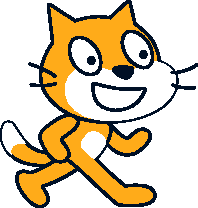
\includegraphics[height=3.9cm]{gato_a.pdf}};}
\newcommand{\gatinhob}{\fill[ink,opacity=.14] (0,-.05) ellipse (1.1 and .18);
\node[anchor=south,inner sep=0pt,transform shape] at (0,.05) {
\includegraphics[height=3.9cm]{gato_b.pdf}};}

% Posiciona um adesivo: \put{x}{y}{escala}{rotacao}{comando}
\newcommand{\colocar}[5]{\begin{scope}[shift={(#1,#2)},scale=#3,rotate=#4]#5\end{scope}}

% --- Fundo de todas as paginas ---
\newcommand{\fundopagina}{%
  \begin{tikzpicture}
    \fill[paper] (0,0) rectangle (\paperwidth,\paperheight);
    \foreach \x in {0,.5,...,21}{\draw[gridc,line width=.3pt] (\x cm,0) -- (\x cm,\paperheight);}
    \foreach \y in {0,.5,...,30}{\draw[gridc,line width=.3pt] (0,\y cm) -- (\paperwidth,\y cm);}
    \ifodd\value{page}
      \colocar{20.3}{28.9}{.95}{15}{\stkgear[scMotion]}
      \colocar{19.0}{29.2}{.6}{-10}{\stkgear[scControl]}
      \colocar{20.5}{27.7}{.5}{0}{\stkbolt}
      \colocar{.9}{1.1}{.75}{-12}{\stkbulb}
      \colocar{2.2}{.7}{.5}{20}{\stkstar[scEvents]}
    \else
      \colocar{.7}{28.9}{.95}{-15}{\stkgear[scLooks]}
      \colocar{2.0}{29.2}{.6}{10}{\stkgear[scControl]}
      \colocar{.5}{27.7}{.5}{0}{\stkbolt}
      \colocar{20.1}{1.1}{.75}{12}{\stkbulb}
      \colocar{18.8}{.7}{.5}{-20}{\stkstar[scEvents]}
    \fi
  \end{tikzpicture}}
\AddToShipoutPictureBG{\AtPageLowerLeft{\fundopagina}}

%----------------------------------------------------------------------------------------
%	BLOCOS DO SCRATCH (para desenhar codigo no livro)
%----------------------------------------------------------------------------------------

% --- Pecas inline (encaixes redondos, menus, booleanos, variaveis) ---
\newcommand{\entrada}[1]{\tikz[baseline=(e.base)]\node(e)[fill=white,rounded corners=7pt,text=ink,inner xsep=5pt,inner ysep=2pt,minimum width=17pt,font=\sffamily\bfseries\small]{#1};}
\newcommand{\menu}[1]{\tikz[baseline=(e.base)]\node(e)[fill=black!20,rounded corners=3pt,text=white,inner xsep=5pt,inner ysep=2pt,font=\sffamily\bfseries\small]{#1\,\scriptsize$\blacktriangledown$};}
\newcommand{\variavel}[1]{\tikz[baseline=(e.base)]\node(e)[fill=scVariables,draw=scVariables!60!black,line width=.7pt,rounded corners=7pt,text=white,inner xsep=5pt,inner ysep=2pt,font=\sffamily\bfseries\small]{#1};}
\newcommand{\reporter}[2][scOperators]{\tikz[baseline=(e.base)]\node(e)[fill=#1,draw=#1!60!black,line width=.7pt,rounded corners=7pt,text=white,inner xsep=5pt,inner ysep=2pt,font=\sffamily\bfseries\small]{#2};}
\newcommand{\booleano}[1]{\tikz[baseline=(e.base)]\node(e)[chamfered rectangle,chamfered rectangle xsep=6pt,chamfered rectangle ysep=6pt,fill=scOperators,draw=scOperators!60!black,line width=.7pt,text=white,inner xsep=3pt,inner ysep=1pt,minimum height=17pt,font=\sffamily\bfseries\small]{#1};}
\newcommand{\bandeira}{\tikz[baseline=-1pt]{\draw[line width=1.4pt,white,line cap=round] (0,-3pt)--(0,10pt);\fill[scOperators,draw=white,line width=.5pt] (0,10pt)--(10pt,7.5pt)--(0,4pt)--cycle;}}

% --- Bloco solto, inline no texto: \bloco[cor]{texto} ---
\newcommand{\bloco}[2][scMotion]{\tikz[baseline=(b.base)]\node(b)[fill=#1,draw=#1!60!black,line width=.8pt,rounded corners=3pt,text=white,inner xsep=7pt,inner ysep=4pt,font=\sffamily\bfseries\small]{#2};}

% --- Pilhas de blocos (ambiente 'pilha') ---
\newdimen\sbx \newdimen\sby \newdimen\sbnw \newcount\sblev
\newcommand{\sbw}{310pt}
\tikzset{sbnode/.style={anchor=north west,inner xsep=9pt,inner ysep=0pt,align=left,text=white,font=\sffamily\bfseries\small,line width=.9pt,rounded corners=3pt}}

\newcommand{\sbtabdraw}[3]{%
  \fill[#1] (#2+10pt,#3) -- ++(3pt,-4pt) -- ++(14pt,0) -- ++(3pt,4pt) -- cycle;
  \draw[#1!60!black,line width=.9pt] (#2+10pt,#3) -- ++(3pt,-4pt) -- ++(14pt,0) -- ++(3pt,4pt);
  \draw[#1,line width=1.5pt] (#2+11.5pt,#3) -- ++(17pt,0);}
\def\sbpend{}
\newcommand{\sbsettab}[1]{\edef\sbpend{\noexpand\sbtabdraw{#1}{\the\sbx}{\the\sby}}}
\newcommand{\sbplace}[3]{%
  \sbnw=\sbw \advance\sbnw by -\sbx \advance\sbnw by -18pt
  \node[sbnode,fill=#1,draw=#1!60!black,minimum height=#2,text width=\sbnw] at (\the\sbx,\the\sby) {#3};
  \sbpend\def\sbpend{}%
  \advance\sby by -#2\relax}

% bloco comum
\newcommand{\bk}[2][scMotion]{\sbplace{#1}{24pt}{#2}\sbsettab{#1}}
% bloco de chapeu (eventos)
\newcommand{\sbh}[2][scEvents]{%
  \sbplace{#1}{32pt}{#2}%
  \draw[fill=#1,draw=#1!60!black,line width=.9pt] (0,0) arc[start angle=180,end angle=0,x radius=46pt,y radius=15pt] -- cycle;
  \draw[#1,line width=1.6pt] (1.2pt,0)--(90.8pt,0);
  \sbsettab{#1}}
% bloco em C (repita, sempre, se...)
\newcommand{\sbc}[2][scControl]{%
  \advance\sblev by 1
  \sbplace{#1}{36pt}{#2}%
  \expandafter\xdef\csname sbcc\the\sblev\endcsname{#1}%
  \expandafter\xdef\csname sbcy\the\sblev\endcsname{\the\sby}%
  \advance\sbx by 14pt
  \sbsettab{#1}}
\newcommand{\sbarm}{%
  \edef\sbcol{\csname sbcc\the\sblev\endcsname}%
  \fill[\sbcol] (\the\sbx-14pt,\csname sbcy\the\sblev\endcsname) rectangle (\the\sbx,\the\sby);
  \draw[\sbcol!60!black,line width=.9pt] (\the\sbx-14pt,\csname sbcy\the\sblev\endcsname)--(\the\sbx-14pt,\the\sby) (\the\sbx,\csname sbcy\the\sblev\endcsname)--(\the\sbx,\the\sby);}
\newcommand{\sbcelse}[1]{%
  \sbarm
  \advance\sbx by -14pt
  \edef\sbcol{\csname sbcc\the\sblev\endcsname}%
  \sbplace{\sbcol}{26pt}{#1}%
  \expandafter\xdef\csname sbcy\the\sblev\endcsname{\the\sby}%
  \advance\sbx by 14pt
  \sbsettab{\sbcol}}
\newcommand{\sbcend}[1][]{%
  \sbarm
  \advance\sbx by -14pt
  \edef\sbcol{\csname sbcc\the\sblev\endcsname}%
  \sbplace{\sbcol}{22pt}{#1}%
  \sbsettab{\sbcol}%
  \advance\sblev by -1 }

\newenvironment{pilha}{%
  \par\medskip\noindent\sbx=0pt \sby=0pt \sblev=0 \def\sbpend{}%
  \begin{tikzpicture}[baseline=(current bounding box.north)]}{%
  \sbpend\end{tikzpicture}\par\medskip}

%----------------------------------------------------------------------------------------
%	CAIXAS COLORIDAS (equivalentes aos teoremas/exercicios do template)
%----------------------------------------------------------------------------------------

\newcommand{\icolampada}{\tikz[baseline=-2pt,scale=.3,transform shape]{\stkbulb}}
\newcommand{\icoestrela}{\tikz[baseline=-2pt,scale=.3,transform shape]{\stkstar}}
\newcommand{\icobug}{\tikz[baseline=-2pt,scale=.3,transform shape]{\stkbug}}
\newcommand{\icoraio}{\tikz[baseline=-2pt,scale=.3,transform shape]{\stkbolt}}
\newcommand{\icoengrenagem}{\tikz[baseline=-2pt,scale=.3,transform shape]{\stkgear}}
\newcommand{\icocheck}{\tikz[baseline=-2pt]{\draw[white,line width=2pt,line cap=round,line join=round] (0,0)--(3pt,-3.5pt)--(9pt,4pt);}}

\tcbset{
  caixa/.style={enhanced,breakable,arc=8pt,boxrule=1.5pt,colframe=ink,colback=white,
    fonttitle=\sffamily\bfseries,coltitle=white,top=19pt,bottom=8pt,left=10pt,right=10pt,
    before skip=18pt,after skip=12pt,
    attach boxed title to top left={xshift=14pt,yshift=-\tcboxedtitleheight/2-2pt},
    boxed title style={colback=#1,colframe=ink,boxrule=1.2pt,arc=7pt,top=3pt,bottom=3pt},
    drop shadow=ink!22},
}

% Missao (laranja) -- objetivo / tarefa principal
\newtcolorbox{missao}[1][Missão]{caixa=scControl,colback=scControl!9,title={\icoestrela\ #1}}
% Dica (amarelo)
\newtcolorbox{dica}[1][Dica]{caixa=scEvents,colback=scEvents!10,coltitle=ink,title={\icolampada\ #1}}
% Cuidado / Bug (roxo com fita de perigo)
\newtcolorbox{cuidado}[1][Cuidado com o Bug!]{caixa=scLooks,colback=scLooks!7,title={\icobug\ #1},
  overlay={\fill[pattern=north east lines,pattern color=ink] ([xshift=60pt]frame.south west) rectangle ([yshift=-5pt]frame.south east);}}
% Vocabulario (azul)
\newtcolorbox{vocabulario}[1][Vocabulário]{caixa=scMotion,colback=scMotion!8,title={\icoengrenagem\ #1}}
% Curiosidade (azul claro)
\newtcolorbox{curiosidade}[1][Você sabia?]{caixa=scSensing,colback=scSensing!10,title={\icoraio\ #1}}
% Pense assim (analogia com a vida real)
\newtcolorbox{pensaassim}[1][Pense assim]{caixa=scSound,colback=scSound!9,title={\icolampada\ #1}}
% Objetivos do capitulo (verde)
\newtcolorbox{objetivos}[1][Nesta missão você vai aprender]{caixa=scOperators,colback=scOperators!9,title={\icoestrela\ #1}}
% Definicao simples, estilo "cartao" tracejado
\newtcolorbox{definicao}[1][]{enhanced,arc=6pt,colback=white,frame hidden,boxrule=0pt,overlay={\draw[ink!70,line width=1.1pt,dash pattern=on 5pt off 3pt,rounded corners=6pt] (frame.south west) rectangle (frame.north east);},
  top=6pt,bottom=6pt,before skip=10pt,after skip=10pt,title={#1},fonttitle=\sffamily\bfseries,coltitle=ink,colbacktitle=white,
  attach title to upper={\par\smallskip}}
% Area de codigo (figura com pilhas de blocos)
\newtcolorbox{codigo}[1][]{enhanced,breakable,arc=8pt,colback=white,colframe=ink!55,boxrule=1.1pt,
  top=6pt,bottom=6pt,before skip=10pt,after skip=10pt,title={#1},fonttitle=\sffamily\bfseries\small,coltitle=ink,colbacktitle=ink!8,
  attach boxed title to top left={xshift=10pt,yshift=-\tcboxedtitleheight/2},boxed title style={arc=5pt,boxrule=.8pt,colframe=ink!55},
  halign=left}
% Exercicio (numerado por capitulo, roxo)
\newtcolorbox[auto counter,number within=chapter]{exercicio}[1][]{caixa=scLooks,colback=scLooks!6,
  title={\icolampada\ Exercício~\thetcbcounter\if\relax\detokenize{#1}\relax\else:~#1\fi}}
% Desafio (rosa)
\newtcolorbox[auto counter,number within=chapter]{desafio}[1][]{caixa=scMyBlocks,colback=scMyBlocks!8,
  title={\icoestrela\ Desafio~\thetcbcounter\if\relax\detokenize{#1}\relax\else:~#1\fi}}
% Resolucao (verde)
\newtcolorbox{resolucaobox}[1][Resolução]{caixa=scOperators,colback=scOperators!9,title={\icocheck\ #1}}

% Resolucoes podem ser ligadas/desligadas em main.tex (\solucoestrue / \solucoesfalse)
\newif\ifsolucoes
\AtBeginDocument{%
  \ifsolucoes
    \specialcomment{solucao}{\begin{resolucaobox}}{\end{resolucaobox}}
  \else
    \excludecomment{solucao}
  \fi}

% Passo a passo com bolinhas numeradas
\newcommand{\bolinha}[1]{\tikz[baseline=(n.base)]\node(n)[circle,fill=\chapcolorname,draw=ink,line width=.7pt,text=white,inner sep=0pt,minimum size=15pt,font=\sffamily\bfseries\small]{#1};}
\newcommand{\estrelinha}{\tikz[baseline=-.4ex,scale=.28,transform shape]{\stkstar}}
\newlist{passos}{enumerate}{1}
\setlist[passos]{label={\protect\bolinha{\arabic*}},leftmargin=28pt,itemsep=5pt}
% Lista de itens com estrelinha
\setlist[itemize,1]{label={\protect\estrelinha},leftmargin=22pt,itemsep=3pt}

%----------------------------------------------------------------------------------------
%	TITULOS: CAPITULOS, SECOES
%----------------------------------------------------------------------------------------

\usepackage{titlesec}
\usepackage{etoolbox}

\newcommand{\setchapcolor}{%
  \ifcase\numexpr\value{chapter}-5*(\value{chapter}/5)\relax
    \gdef\chapcolorname{scOperators}\or % 1
    \gdef\chapcolorname{scControl}\or   % 2
    \gdef\chapcolorname{scMotion}\or    % 3
    \gdef\chapcolorname{scLooks}\or     % 4
    \gdef\chapcolorname{scMyBlocks}\else\gdef\chapcolorname{scControl}\fi}

% Faixa colorida no topo da pagina do capitulo
\newcommand{\faixacapitulo}[2]{% #1 = rotulo (ex: Capitulo 1), #2 = titulo
  \begin{tikzpicture}[remember picture,overlay,shift={(current page.north west)}]
    \fill[\chapcolorname] (0,0) rectangle (\paperwidth,-6.2cm);
    \fill[white,opacity=.18] (\paperwidth-2cm,-6.2cm) circle(2.4cm) (3cm,-6.2cm) circle(1.5cm);
    \draw[ink,line width=1.6pt] (0,-6.2cm)--(\paperwidth,-6.2cm);
    \colocar{18.6cm}{-1.3cm}{.9}{10}{\stkgear[white]}
    \colocar{17.2cm}{-.8cm}{.55}{0}{\stkstar}
    \colocar{19.7cm}{-3.2cm}{.6}{-15}{\stkbolt}
    \colocar{16.8cm}{-5.4cm}{.6}{15}{\stkbug}
    \if\relax\detokenize{#1}\relax\else\node[anchor=west,fill=white,draw=ink,line width=1.3pt,rounded corners=10pt,inner xsep=12pt,inner ysep=4pt,
      font=\sffamily\bfseries\large,text=ink] at (2.6cm,-1.9cm) {#1};\fi
    \node[anchor=west,text width=12.2cm,align=left,text=white,font=\fontsize{30}{33}\selectfont\sffamily\bfseries] at (2.6cm,-3.9cm) {#2};
  \end{tikzpicture}}

% Capitulos: mesmo metodo do template original (redefine os "makechapterhead")
\makeatletter
\def\@makechapterhead#1{\setchapcolor\faixacapitulo{\chaptername\ \thechapter}{#1}\par\vspace*{3.8cm}}
\def\@makeschapterhead#1{\gdef\chapcolorname{scMotion}\faixacapitulo{}{#1}\par\vspace*{3.8cm}}
\makeatother

\titleformat{\section}{\sffamily\bfseries\Large\color{ink}}
  {\tikz[baseline=(n.base)]\node(n)[fill=\chapcolorname,draw=ink,line width=.8pt,text=white,rounded corners=5pt,inner xsep=6pt,inner ysep=3pt,font=\sffamily\bfseries\normalsize]{\thesection};}{.7em}{}
\titlespacing*{\section}{0pt}{22pt plus 4pt minus 2pt}{8pt}
\titleformat{\subsection}{\sffamily\bfseries\large\color{\chapcolorname!85!black}}
  {\tikz[baseline=-.5ex]\fill[\chapcolorname,draw=ink,line width=.6pt] (0,0) circle(4pt);}{.6em}{}
\titlespacing*{\subsection}{0pt}{14pt plus 3pt minus 2pt}{5pt}
\titleformat{\subsubsection}{\sffamily\bfseries\normalsize\color{ink}}{}{0pt}{}
\titlespacing*{\subsubsection}{0pt}{10pt}{3pt}

%----------------------------------------------------------------------------------------
%	CABECALHO / RODAPE
%----------------------------------------------------------------------------------------

\usepackage{fancyhdr}
\pagestyle{fancy}
\setlength{\headheight}{26pt}
\renewcommand{\chaptermark}[1]{\markboth{\chaptername\ \thechapter\ ·\ #1}{}}
\renewcommand{\sectionmark}[1]{\markright{\thesection\ #1}{}}
\fancyhf{}
\newcommand{\selopagina}{\tikz[baseline=(p.base)]\node(p)[circle,fill=\chapcolorname,draw=ink,line width=.9pt,text=white,minimum size=.8cm,inner sep=0pt,font=\sffamily\bfseries]{\thepage};}
\newcommand{\cabecalhotexto}{\textcolor{ink!75}{\sffamily\footnotesize \leftmark \quad|\quad \rightmark}}
\newcommand{\rodapetexto}[1]{\textcolor{ink!75}{\sffamily\footnotesize #1}}
\fancyhead[L]{\cabecalhotexto}
\fancyhead[R]{\selopagina}
\fancyfoot[L]{\rodapetexto{Universidade de Rio Verde}}
\fancyfoot[C]{\rodapetexto{Engenharia de Software}}
\fancyfoot[R]{\rodapetexto{Programação com Scratch}}
\renewcommand{\footrule}{\vskip-\footruleskip\vskip-2.4pt{\color{\chapcolorname}\hrule height 2.4pt width\headwidth}\vskip\footruleskip}
\renewcommand{\footrulewidth}{2.4pt}
\fancypagestyle{plain}{\fancyhf{}%
  \fancyhead[R]{\selopagina}%
  \fancyfoot[L]{\rodapetexto{Universidade de Rio Verde}}%
  \fancyfoot[C]{\rodapetexto{Engenharia de Software}}%
  \fancyfoot[R]{\rodapetexto{Programação com Scratch}}%
  \renewcommand{\headrulewidth}{0pt}%
  \renewcommand{\footrulewidth}{2.4pt}}
\renewcommand{\headrule}{{\color{\chapcolorname}\hrule height 2.4pt width\headwidth}\vskip-2.4pt}
\renewcommand{\headrulewidth}{2.4pt}

%----------------------------------------------------------------------------------------
%	SUMARIO
%----------------------------------------------------------------------------------------

\usepackage{titletoc}
\contentsmargin{0cm}
\titlecontents{part}[0cm]{\addvspace{18pt}\sffamily\bfseries\Large\color{scLooks!85!black}}{Parte \thecontentslabel\ ---\ }{}{}
\titlecontents{chapter}[2.3em]{\addvspace{9pt}\sffamily\bfseries\large}
  {\color{scControl!90!black}\contentslabel{2.3em}}{\hspace*{-2.3em}}{\ \titlerule*[5pt]{.}\contentspage}
\titlecontents{section}[4.6em]{\sffamily\small}{\contentslabel{2.3em}}{}{\ \titlerule*[4pt]{.}\contentspage}
\setcounter{tocdepth}{1}
\setcounter{secnumdepth}{2}

%----------------------------------------------------------------------------------------
%	PAGINA DE PARTE (separador colorido)
%----------------------------------------------------------------------------------------

\newcommand{\parte}[2]{% #1 = titulo, #2 = subtitulo
  \cleardoublepage
  \refstepcounter{part}%
  \addcontentsline{toc}{part}{\protect\numberline{\thepart}#1}%
  \thispagestyle{empty}%
  \begin{tikzpicture}[remember picture,overlay,shift={(current page.south west)}]
    \fill[scLooks!22] (0,0) rectangle (\paperwidth,\paperheight);
    \foreach \x in {0,.5,...,21}{\draw[white,opacity=.55,line width=.3pt] (\x cm,0) -- (\x cm,\paperheight);}
    \foreach \y in {0,.5,...,30}{\draw[white,opacity=.55,line width=.3pt] (0,\y cm) -- (\paperwidth,\y cm);}
    \node[text=scLooks!55,font=\fontsize{210}{210}\selectfont\sffamily\bfseries] at (10.5,23) {\Roman{part}};
    \node[fill=white,draw=ink,line width=2pt,rounded corners=18pt,inner sep=20pt,text width=13cm,align=center,
      font=\sffamily,drop shadow={ink!25}] at (10.5,15.2)
      {{\Large\bfseries\color{scMotion!90!black}Parte \Roman{part}}\\[6pt]{\fontsize{30}{34}\selectfont\bfseries\color{ink}#1}\\[8pt]{\large\color{ink!80}#2}};
    \colocar{4}{1.8}{1.9}{0}{\robozinho}
    \colocar{17}{1.8}{1.8}{0}{\gatinhob}
    \colocar{2.5}{26}{1.3}{15}{\stkgear[scMotion]}
    \colocar{18.5}{27}{1.5}{-10}{\stkgear[scControl]}
    \colocar{9.5}{27.7}{1}{10}{\stkstar}
    \colocar{19}{15.5}{.9}{0}{\stkbulb}
    \colocar{2}{16.5}{.9}{0}{\stkbug}
  \end{tikzpicture}
  \clearpage}

%----------------------------------------------------------------------------------------
%	CAPA
%----------------------------------------------------------------------------------------

\newcommand{\capalivro}[3]{% #1 = subtitulo, #2 = autor, #3 = faixa inferior
  \thispagestyle{empty}
  \begin{tikzpicture}[remember picture,overlay,shift={(current page.south west)}]
    % titulo em letras coloridas
    \foreach \l/\c/\r [count=\i from 0] in {S/scControl/-4, c/scMotion/3, r/scLooks/-3, a/scOperators/4, t/scMyBlocks/-4, c/scEvents/3, h/scSensing/-3}{
      \node[rotate=\r,text=ink,font=\fontsize{96}{96}\selectfont\sffamily\bfseries] at (3.1+\i*2.4+.12,22.9-.12) {\l};
      \node[rotate=\r,text=\c,font=\fontsize{96}{96}\selectfont\sffamily\bfseries] at (3.1+\i*2.4,22.9) {\l};}
    \node[fill=white,draw=ink,line width=1.6pt,rounded corners=16pt,inner xsep=18pt,inner ysep=9pt,
      font=\Large\sffamily\bfseries,text width=14cm,align=center,drop shadow={ink!25}] at (10.5,19.9) {#1};
    \colocar{4.7}{7.4}{2.5}{0}{\robozinho}
    \colocar{16.3}{7.4}{2.4}{0}{\gatinho}
    \colocar{10.5}{14.2}{1.3}{8}{\stkstar}
    \colocar{9.2}{16.6}{.9}{-12}{\stkstar[scMyBlocks]}
    \colocar{12.2}{16.9}{.8}{14}{\stkstar[scMotion]}
    \colocar{1.7}{18.2}{1.4}{10}{\stkgear[scMotion]}
    \colocar{19.2}{18.3}{1.5}{-10}{\stkgear[scControl]}
    \colocar{1.8}{25.6}{1.2}{-15}{\stkbulb}
    \colocar{19.2}{26.2}{1.1}{15}{\stkbolt}
    \colocar{10.6}{10.0}{1.4}{0}{\stkbug}
    \colocar{9.4}{12.0}{1.0}{0}{\stkbug[scMyBlocks]}
    \colocar{2.0}{4.9}{.9}{15}{\stkbolt}
    \colocar{19.2}{5.0}{.9}{-15}{\stkstar[scMotion]}
    % faixa inferior
    \node[fill=scMotion,draw=ink,line width=1.8pt,rounded corners=14pt,text=white,inner xsep=24pt,inner ysep=10pt,
      font=\Large\sffamily\bfseries,drop shadow={ink!25}] at (10.5,3.6) {#3};
    \node[font=\normalsize\sffamily\bfseries,text=ink,align=center,text width=15cm] at (10.5,1.6) {#2};
  \end{tikzpicture}
  \clearpage}

%----------------------------------------------------------------------------------------
%	HYPERLINKS
%----------------------------------------------------------------------------------------

\usepackage{hyperref}
\hypersetup{hidelinks,colorlinks=false,breaklinks=true,pdftitle={Scratch - Guia Completo},pdfauthor={Autor}}


\newcommand{\versaodolivro}{1.0.0}
\newcommand{\datadaversao}{18 de novembro de 2026}
\solucoestrue
\hypersetup{pdftitle={Scratch - O Guia Completo - v\versaodolivro}}

\begin{document}

%----------------------------------------------------------------------------------------
%	CAPA
%----------------------------------------------------------------------------------------

\capalivro
  {O Guia Completo\\[2pt]\normalfont\normalsize do zero ao seu primeiro jogo!}
  {Gilberto Aparecido Dias Junior \\ Maycon Garcia Silva \\ Vinicius Félix de Paula}
  {Missões · Exercícios · Resoluções · v\versaodolivro}

%----------------------------------------------------------------------------------------
%	FICHA / DIREITOS
%----------------------------------------------------------------------------------------

~\vfill
\thispagestyle{empty}
\noindent\textbf{Scratch: o Guia Completo}\\
Copyright \copyright\ \the\year\ Gilberto Aparecido Dias Junior, Maycon Garcia Silva e Vinicius Félix de Paula\\[6pt]
Scratch é um projeto do Scratch Foundation, em colaboração com o Lifelong Kindergarten Group do MIT Media Lab. Mais informações em \texttt{scratch.mit.edu}.\\[6pt]
\textit{Primeira edição. Versão \versaodolivro, \datadaversao.}
\clearpage

%----------------------------------------------------------------------------------------
%	SUMARIO
%----------------------------------------------------------------------------------------

\pagestyle{empty}
\tableofcontents
\cleardoublepage
\pagestyle{fancy}

%----------------------------------------------------------------------------------------
%	CONTEUDO
%----------------------------------------------------------------------------------------

\parte{Primeiros Passos}{Conheça o Scratch e mande o gatinho andar!}

\chapter{Bem-vindo ao Scratch!}

\begin{objetivos}
\begin{itemize}
\item Descobrir o que é o Scratch e para que ele serve;
\item Conhecer as partes da tela: palco, atores e blocos;
\item Montar e rodar o seu primeiro programa.
\end{itemize}
\end{objetivos}

\section{O que é o Scratch?}

O \textbf{Scratch} é uma linguagem de programação feita para quem está começando. Em vez de escrever códigos difíceis, você \textbf{encaixa blocos coloridos}, como se fossem peças de quebra-cabeça. Com eles dá para criar histórias, animações, músicas e até jogos!

\begin{vocabulario}
\textbf{Programar} é dar ordens, passo a passo, para o computador. Um conjunto de ordens se chama \textbf{programa} (ou \textbf{código}).
\end{vocabulario}

Cada bloco é uma ordem. Veja como é um programa pequeno:

\begin{codigo}[Meu primeiro programa]
\begin{pilha}
\sbh[scEvents]{quando \bandeira\ for clicado}
\bk[scMotion]{mova \entrada{10} passos}
\bk[scLooks]{diga \entrada{Olá!} por \entrada{2} segundos}
\end{pilha}
\end{codigo}

\begin{dica}
Os blocos só se encaixam de cima para baixo, e o computador executa uma ordem de cada vez, \textbf{na ordem em que estão empilhadas}.
\end{dica}

\section{Sequência: a ordem importa!}

Uma lista de ordens colocadas uma depois da outra se chama \textbf{sequência de instruções}. O computador é muito obediente, mas não pensa por conta própria: ele faz \textbf{exatamente} o que está escrito, \textbf{na ordem} em que está escrito.

\begin{pensaassim}[Pense assim: a receita de bolo]
Para fazer um bolo, você segue uma receita: \emph{1) misture os ingredientes, 2) coloque na forma, 3) asse no forno}. Se você assar \textbf{antes} de misturar, o bolo não sai! O mesmo vale para um programa: cada bloco é um passo da receita, e a ordem muda o resultado.
\end{pensaassim}

\begin{pensaassim}[Pense assim: se vestir]
Você coloca a \textbf{meia} e só depois o \textbf{sapato}. Se inverter a ordem, o resultado fica engraçado (e errado!). Na programação, trocar dois blocos de lugar pode mudar tudo.
\end{pensaassim}

Veja dois programas com os \textbf{mesmos blocos}, mas em ordens diferentes:

\begin{codigo}[Ordem certa]
\begin{pilha}
\sbh[scEvents]{quando \bandeira\ for clicado}
\bk[scMotion]{mova \entrada{50} passos}
\bk[scLooks]{diga \entrada{Cheguei!} por \entrada{2} segundos}
\end{pilha}
\end{codigo}

\begin{codigo}[Ordem trocada]
\begin{pilha}
\sbh[scEvents]{quando \bandeira\ for clicado}
\bk[scLooks]{diga \entrada{Cheguei!} por \entrada{2} segundos}
\bk[scMotion]{mova \entrada{50} passos}
\end{pilha}
\end{codigo}

No primeiro, o gatinho anda e depois diz ``Cheguei!''. No segundo, ele diz ``Cheguei!'' \textbf{antes} de andar, ou seja, ainda nem chegou! Os blocos são iguais, mas o programa conta uma história diferente.

\begin{dica}[Teste a sequência]
Quando um programa não faz o que você queria, leia os blocos de cima para baixo, um de cada vez, fingindo que você é o computador. Muitas vezes o erro é só uma ordem trocada.
\end{dica}

\section{As cores dos blocos}

Cada cor de bloco tem um trabalho diferente. Assim fica fácil achar o que você precisa!

\begin{center}
\renewcommand{\arraystretch}{1.7}
\begin{tabular}{@{}lll@{}}
\bloco[scMotion]{Movimento} & mexe o ator pela tela & \small\textit{mova, gire, vá para}\\
\bloco[scLooks]{Aparência} & muda o visual e as falas & \small\textit{diga, mude de fantasia}\\
\bloco[scSound]{Som} & toca sons e músicas & \small\textit{toque o som}\\
\bloco[scEvents]{Eventos} & começa o programa & \small\textit{quando clicar na bandeira}\\
\bloco[scControl]{Controle} & repete e decide & \small\textit{repita, se\ldots então}\\
\bloco[scSensing]{Sensores} & percebe o que acontece & \small\textit{tocando em, tecla pressionada}\\
\bloco[scOperators]{Operadores} & faz contas e comparações & \small\textit{+, $-$, $>$, aleatório}\\
\bloco[scVariables]{Variáveis} & guarda informações & \small\textit{pontos, vidas}\\
\bloco[scMyBlocks]{Meus Blocos} & blocos criados por você & \small\textit{seus próprios comandos}\\
\end{tabular}
\end{center}

\section{Conhecendo a tela}

Quando você abre o Scratch, vê quatro áreas principais:

\begin{center}
\begin{tikzpicture}[x=1cm,y=1cm,font=\sffamily\small]
  % janela
  \draw[fill=white,draw=ink,line width=1.4pt,rounded corners=8pt] (0,0) rectangle (13,7.2);
  \fill[scMotion] (0,6.5) [rounded corners=8pt] rectangle (13,7.2);
  % paleta de blocos
  \draw[fill=scMotion!12,draw=ink,line width=1pt] (.3,.3) rectangle (3.2,6.2);
  \foreach \y/\c in {5.5/scMotion,4.8/scLooks,4.1/scSound,3.4/scEvents,2.7/scControl}{\fill[\c,draw=ink,rounded corners=2pt] (.55,\y) rectangle (2.95,\y+.45);}
  % area de codigo
  \draw[fill=white,draw=ink,line width=1pt] (3.4,.3) rectangle (8.2,6.2);
  \fill[scEvents,draw=ink,rounded corners=2pt] (4,5.2) rectangle (6.4,5.65);
  \fill[scMotion,draw=ink,rounded corners=2pt] (4,4.7) rectangle (6.4,5.15);
  \fill[scLooks,draw=ink,rounded corners=2pt] (4,4.2) rectangle (6.4,4.65);
  % palco
  \draw[fill=white,draw=ink,line width=1pt] (8.4,2.6) rectangle (12.7,6.2);
  \begin{scope}[shift={(10.55,3.5)},scale=.42]\gatinho\end{scope}
  % lista de atores
  \draw[fill=scLooks!10,draw=ink,line width=1pt] (8.4,.3) rectangle (12.7,2.4);
  \draw[fill=white,draw=ink,rounded corners=3pt] (8.7,.6) rectangle (9.9,2.1);
  \begin{scope}[shift={(9.3,.85)},scale=.2]\gatinho\end{scope}
  % rotulos
  \node[fill=scMotion,draw=ink,text=white,rounded corners=4pt,inner sep=3pt,font=\sffamily\bfseries\footnotesize] at (1.75,-.55) {1. Paleta de blocos};
  \node[fill=scControl,draw=ink,text=white,rounded corners=4pt,inner sep=3pt,font=\sffamily\bfseries\footnotesize] at (5.8,-.55) {2. Área de código};
  \node[fill=scOperators,draw=ink,text=white,rounded corners=4pt,inner sep=3pt,font=\sffamily\bfseries\footnotesize] at (10.5,-.55) {3. Palco e 4. Atores};
\end{tikzpicture}
\end{center}

\begin{description}[leftmargin=!,labelwidth=3.4cm,style=nextline]
\item[\textbf{1. Paleta de blocos}] Fica na esquerda. É a ``caixa de peças'' com todos os blocos, separados por cor.
\item[\textbf{2. Área de código}] Fica no meio. É onde você arrasta e encaixa os blocos para montar o programa.
\item[\textbf{3. Palco}] Fica no alto, à direita. É onde a ação acontece! Tudo o que o seu programa faz aparece aqui.
\item[\textbf{4. Atores}] Fica embaixo do palco. Aqui moram os personagens (o gatinho é o ator inicial).
\end{description}

\begin{vocabulario}[Vocabulário: ator e palco]
Em Scratch, cada personagem ou objeto é um \textbf{ator} (em inglês, \textit{sprite}). O cenário onde eles aparecem é o \textbf{palco} (\textit{stage}).
\end{vocabulario}

\section{Seu primeiro programa}

\begin{missao}[Missão 1: Faça o gatinho falar!]
Faça o gatinho andar um pouquinho e dizer ``Olá!'' quando você clicar na bandeira verde.
\end{missao}

\begin{passos}
\item Clique na categoria \bloco[scEvents]{Eventos} e arraste \bloco[scEvents]{quando \bandeira\ for clicado} para a área de código.
\item Na categoria \bloco[scMotion]{Movimento}, arraste \bloco[scMotion]{mova \entrada{10} passos} e encaixe embaixo do primeiro bloco.
\item Em \bloco[scLooks]{Aparência}, arraste \bloco[scLooks]{diga \entrada{Olá!} por \entrada{2} segundos} e encaixe por último.
\item Clique na \bandeira\ \textbf{bandeira verde} acima do palco e veja a mágica acontecer!
\end{passos}

\begin{cuidado}
Se nada acontecer, confira se os blocos estão \textbf{encaixados} (colados uns nos outros). Blocos soltos não funcionam!
\end{cuidado}

\begin{curiosidade}
O Scratch foi criado em 2007 por um grupo de pesquisadores do MIT, nos Estados Unidos. Hoje milhões de crianças no mundo todo usam o Scratch!
\end{curiosidade}

\section{Hora de praticar}

\begin{exercicio}[Troque a fala]
Mude o texto do bloco \bloco[scLooks]{diga \entrada{Olá!} por \entrada{2} segundos} para dizer o seu nome, por 3 segundos.
\end{exercicio}

\begin{solucao}
Clique no texto \entrada{Olá!} e digite o seu nome. Depois clique no número \entrada{2} e troque por \entrada{3}.
\begin{pilha}
\sbh[scEvents]{quando \bandeira\ for clicado}
\bk[scMotion]{mova \entrada{10} passos}
\bk[scLooks]{diga \entrada{Maria} por \entrada{3} segundos}
\end{pilha}
\end{solucao}

\begin{exercicio}[Dois passos]
Faça o gatinho andar \textbf{20 passos} em vez de 10 e depois dizer ``Cheguei!''.
\end{exercicio}

\begin{solucao}
\begin{pilha}
\sbh[scEvents]{quando \bandeira\ for clicado}
\bk[scMotion]{mova \entrada{20} passos}
\bk[scLooks]{diga \entrada{Cheguei!} por \entrada{2} segundos}
\end{pilha}
\end{solucao}

\begin{desafio}[Andou, falou, andou]
Faça o gatinho andar 10 passos, dizer ``Oi!'', e depois andar mais 10 passos. Dica: você pode usar o mesmo bloco \bloco[scMotion]{mova \entrada{10} passos} duas vezes.
\end{desafio}

\begin{solucao}
\begin{pilha}
\sbh[scEvents]{quando \bandeira\ for clicado}
\bk[scMotion]{mova \entrada{10} passos}
\bk[scLooks]{diga \entrada{Oi!} por \entrada{2} segundos}
\bk[scMotion]{mova \entrada{10} passos}
\end{pilha}
\end{solucao}

\chapter{Movimento e Direção}

\begin{objetivos}
\begin{itemize}
\item Usar os blocos de \textbf{Movimento} para mexer os atores;
\item Entender o plano do palco com as coordenadas \textbf{x} e \textbf{y};
\item Fazer um ator girar, deslizar e repetir um movimento.
\end{itemize}
\end{objetivos}

\section{Os blocos de movimento}

Os blocos azuis \bloco[scMotion]{Movimento} dizem para onde o ator vai. Os mais usados são:

\begin{center}
\renewcommand{\arraystretch}{1.8}
\begin{tabular}{@{}ll@{}}
\bloco[scMotion]{mova \entrada{10} passos} & anda para a frente \\
\bloco[scMotion]{gire \entrada{15} graus} & vira o ator \\
\bloco[scMotion]{vá para x: \entrada{0} y: \entrada{0}} & vai direto para um ponto \\
\bloco[scMotion]{deslize por \entrada{1} seg até x: \entrada{0} y: \entrada{0}} & vai deslizando até lá \\
\end{tabular}
\end{center}

\begin{dica}
Passos \textbf{negativos} fazem o ator andar para trás! Experimente \bloco[scMotion]{mova \entrada{$-10$} passos}.
\end{dica}

\section{O plano do palco: x e y}

O palco é como um \textbf{papel quadriculado}. Cada lugar tem um endereço com dois números: o \textbf{x} (esquerda--direita) e o \textbf{y} (embaixo--em cima). O centro é o ponto \textbf{(0, 0)}.

\begin{center}
\begin{tikzpicture}[font=\sffamily\small]
  \draw[fill=white,draw=ink,line width=1.3pt,rounded corners=4pt] (-4.8,-3.6) rectangle (4.8,3.6);
  \draw[gridc!70!ink,line width=.4pt] (-4.8,-3.6) grid[step=.6] (4.8,3.6);
  \draw[ink,-{Stealth},line width=1.1pt] (-4.8,0)--(5.1,0) node[right]{\bfseries x};
  \draw[ink,-{Stealth},line width=1.1pt] (0,-3.6)--(0,3.9) node[above]{\bfseries y};
  \node[fill=scMotion,draw=ink,text=white,inner sep=2pt,rounded corners=2pt,font=\sffamily\bfseries\scriptsize] at (-4.4,-.3) {$-240$};
  \node[fill=scMotion,draw=ink,text=white,inner sep=2pt,rounded corners=2pt,font=\sffamily\bfseries\scriptsize] at (4.4,-.3) {$240$};
  \node[fill=scOperators,draw=ink,text=white,inner sep=2pt,rounded corners=2pt,font=\sffamily\bfseries\scriptsize] at (.6,3.3) {$180$};
  \node[fill=scOperators,draw=ink,text=white,inner sep=2pt,rounded corners=2pt,font=\sffamily\bfseries\scriptsize] at (.65,-3.3) {$-180$};
  \fill[scMyBlocks,draw=ink] (2.4,1.8) circle(.13) node[above right,font=\sffamily\bfseries\footnotesize]{(120, 90)};
  \fill[scLooks,draw=ink] (-2.4,-1.2) circle(.13) node[below left,font=\sffamily\bfseries\footnotesize]{($-120$, $-60$)};
  \fill[scEvents,draw=ink] (0,0) circle(.13);
\end{tikzpicture}
\end{center}

\begin{definicao}[Resumo]
\textbf{x} mede \emph{para o lado}: positivo é direita, negativo é esquerda.\\
\textbf{y} mede \emph{para cima}: positivo é para cima, negativo é para baixo.
\end{definicao}

\section{Girando}

O bloco \bloco[scMotion]{gire \entrada{15} graus} vira o ator para a direita. Uma volta completa tem \textbf{360 graus}. Girar 90 graus é um quarto de volta, como a curva de uma esquina.

\begin{missao}[Missão 2: Dança do gatinho]
Faça o gatinho andar, girar, andar de novo e deslizar de volta para o centro do palco.
\end{missao}

\begin{codigo}[Uma solução possível]
\begin{pilha}
\sbh[scEvents]{quando \bandeira\ for clicado}
\bk[scMotion]{mova \entrada{50} passos}
\bk[scMotion]{gire \entrada{90} graus}
\bk[scMotion]{mova \entrada{50} passos}
\bk[scMotion]{deslize por \entrada{1} seg até x: \entrada{0} y: \entrada{0}}
\end{pilha}
\end{codigo}

\section{Repetindo movimentos}

Imagine ter que arrastar o mesmo bloco 4 vezes! Para isso existe o bloco laranja \bloco[scControl]{repita \entrada{4} vezes}. Tudo o que estiver dentro dele é repetido.

\begin{codigo}[Desenhando um quadrado]
\begin{pilha}
\sbh[scEvents]{quando \bandeira\ for clicado}
\sbc[scControl]{repita \entrada{4} vezes}
\bk[scMotion]{mova \entrada{100} passos}
\bk[scMotion]{gire \entrada{90} graus}
\sbcend
\end{pilha}
\end{codigo}

\begin{vocabulario}[Vocabulário: repetição]
Repetir um conjunto de ordens várias vezes se chama \textbf{laço} (em inglês, \textit{loop}). Ele evita que a gente copie blocos sem parar.
\end{vocabulario}

\begin{pensaassim}[Pense assim: escovar os dentes]
Ninguém diz ``mova a escova, mova a escova, mova a escova\ldots'' trinta vezes. Dizemos só: \emph{``escove por 30 movimentos''}. O bloco \bloco[scControl]{repita} faz isso: você escreve o passo \textbf{uma vez} e diz \textbf{quantas vezes} repetir. No quadrado acima, \emph{mova 100 passos e gire 90 graus} é um ``lado'', e o gatinho repete 4 lados.
\end{pensaassim}

\section{Hora de praticar}

\begin{exercicio}[Vá para o canto]
Use um bloco para levar o gatinho até o canto superior direito do palco, no ponto $x=200$, $y=150$.
\end{exercicio}

\begin{solucao}
\begin{pilha}
\sbh[scEvents]{quando \bandeira\ for clicado}
\bk[scMotion]{vá para x: \entrada{200} y: \entrada{150}}
\end{pilha}
\end{solucao}

\begin{exercicio}[Meia-volta]
Faça o gatinho andar 100 passos, dar meia-volta (180 graus) e voltar ao ponto de partida.
\end{exercicio}

\begin{solucao}
Meia-volta é 180 graus. Depois de girar, andar o mesmo tanto traz o gato de volta.
\begin{pilha}
\sbh[scEvents]{quando \bandeira\ for clicado}
\bk[scMotion]{mova \entrada{100} passos}
\bk[scMotion]{gire \entrada{180} graus}
\bk[scMotion]{mova \entrada{100} passos}
\end{pilha}
\end{solucao}

\begin{exercicio}[Triângulo]
Desenhe um triângulo com o gatinho usando \bloco[scControl]{repita}. Dica: em um triângulo com lados iguais, cada giro é de $360 \div 3 = 120$ graus.
\end{exercicio}

\begin{solucao}
\begin{pilha}
\sbh[scEvents]{quando \bandeira\ for clicado}
\sbc[scControl]{repita \entrada{3} vezes}
\bk[scMotion]{mova \entrada{100} passos}
\bk[scMotion]{gire \entrada{120} graus}
\sbcend
\end{pilha}
\end{solucao}

\begin{desafio}[Sua própria figura]
Descubra quantas vezes repetir e quantos graus girar para desenhar um \textbf{hexágono} (6 lados). Dica: $360 \div 6$.
\end{desafio}

\begin{solucao}
Seis lados, então repita 6 vezes, girando $360 \div 6 = 60$ graus a cada lado.
\begin{pilha}
\sbh[scEvents]{quando \bandeira\ for clicado}
\sbc[scControl]{repita \entrada{6} vezes}
\bk[scMotion]{mova \entrada{60} passos}
\bk[scMotion]{gire \entrada{60} graus}
\sbcend
\end{pilha}
\end{solucao}

\chapter{Aparência: Mudando o Visual}

\begin{objetivos}
\begin{itemize}
\item Fazer o ator falar e pensar com balões;
\item Trocar de fantasia para criar movimento;
\item Mudar tamanho, cor e esconder ou mostrar o ator.
\end{itemize}
\end{objetivos}

\section{Falar e pensar}

\begin{pensaassim}[Pense assim: uma história em quadrinhos]
Nos quadrinhos, um balão mostra o que o personagem diz e outro mostra o que ele pensa. No Scratch, você também escolhe o texto e o tipo de balão. Esses balões aparecem na tela: eles não produzem voz.
\end{pensaassim}

Os blocos roxos \bloco[scLooks]{Aparência} cuidam do \textbf{visual} do ator. Os dois mais simples fazem aparecer um balão de fala ou de pensamento:

\begin{center}
\renewcommand{\arraystretch}{1.8}
\begin{tabular}{@{}ll@{}}
\bloco[scLooks]{diga \entrada{Olá!} por \entrada{2} segundos} & fala e depois o balão some \\
\bloco[scLooks]{diga \entrada{Olá!}} & fala e o balão fica na tela \\
\bloco[scLooks]{pense \entrada{Hmm...} por \entrada{2} segundos} & balão de pensamento \\
\end{tabular}
\end{center}

\begin{dica}
Use \bloco[scLooks]{diga \entrada{}} com o texto vazio para apagar um balão que ficou na tela.
\end{dica}

\section{Fantasias}

Cada ator pode ter várias \textbf{fantasias}. Uma fantasia é uma imagem diferente do mesmo ator, como os quadros de um desenho animado. O gatinho já vem com duas: uma de perna aberta e outra de perna fechada.

\begin{vocabulario}[Vocabulário: fantasia]
\textbf{Fantasia} é cada aparência de um ator. Trocar de fantasia depressa dá a sensação de movimento, e isso se chama \textbf{animação}.
\end{vocabulario}

\begin{pensaassim}[Pense assim: trocando de roupa]
Você pode vestir um pijama ou uma roupa de passeio e continuar sendo a mesma pessoa. As fantasias são aparências diferentes do mesmo ator: trocar a fantasia não cria outro personagem.
\end{pensaassim}

\begin{center}
\renewcommand{\arraystretch}{1.8}
\begin{tabular}{@{}ll@{}}
\bloco[scLooks]{próxima fantasia} & passa para a fantasia seguinte \\
\bloco[scLooks]{mude para a fantasia \menu{gato-b}} & escolhe uma fantasia específica \\
\end{tabular}
\end{center}

\begin{missao}[Missão 3: O gatinho que corre]
Faça o gatinho correr pelo palco, alternando as fantasias a cada passo.
\end{missao}

\begin{codigo}[Gatinho andando]
\begin{pilha}
\bk[scEvents]{quando \bandeira\ for clicado}
\sbc[scControl]{repita \entrada{10} vezes}
\bk[scMotion]{mova \entrada{10} passos}
\bk[scLooks]{próxima fantasia}
\bk[scControl]{espere \entrada{0.1} segundos}
\sbcend
\end{pilha}
\end{codigo}

\begin{cuidado}
Sem o bloco \bloco[scControl]{espere \entrada{0.1} segundos}, as fantasias trocam rápido demais e o gatinho parece tremer em vez de correr.
\end{cuidado}

\section{Tamanho, cor e visibilidade}

\begin{pensaassim}[Pense assim: uma foto e um fantoche]
Ao ampliar uma foto ou aplicar um filtro, você muda o tamanho ou as cores da imagem. Os efeitos do ator fazem algo parecido. Já esconder um ator é como colocar um fantoche atrás da cortina: você deixa de vê-lo, mas ele continua no projeto e pode aparecer de novo.
\end{pensaassim}

\begin{center}
\renewcommand{\arraystretch}{1.8}
\begin{tabular}{@{}ll@{}}
\bloco[scLooks]{mude o tamanho para \entrada{150} \%} & define o tamanho exato (100\% é o normal) \\
\bloco[scLooks]{mude o tamanho em \entrada{10}} & cresce (ou encolhe, se for negativo) \\
\bloco[scLooks]{mude o efeito \menu{cor} para \entrada{25}} & troca a cor do ator \\
\bloco[scLooks]{esconda} & o ator some do palco \\
\bloco[scLooks]{mostre} & o ator aparece de novo \\
\end{tabular}
\end{center}

\begin{curiosidade}
Efeitos como \textbf{cor}, \textbf{olho de peixe} e \textbf{mosaico} deixam o ator com cara de filtro de foto! Para voltar ao normal, use o bloco \bloco[scLooks]{tire os efeitos gráficos}.
\end{curiosidade}

\section{Hora de praticar}

\begin{exercicio}[Pensando alto]
Faça o gatinho \textbf{pensar} ``Que dia lindo!'' por 3 segundos e depois \textbf{dizer} ``Vamos brincar!'' por 2 segundos.
\end{exercicio}

\begin{solucao}
\begin{pilha}
\bk[scEvents]{quando \bandeira\ for clicado}
\bk[scLooks]{pense \entrada{Que dia lindo!} por \entrada{3} segundos}
\bk[scLooks]{diga \entrada{Vamos brincar!} por \entrada{2} segundos}
\end{pilha}
\end{solucao}

\begin{exercicio}[Gigante e pequeno]
Faça o gatinho ficar com o dobro do tamanho (200\%), esperar 1 segundo e depois voltar ao tamanho normal (100\%).
\end{exercicio}

\begin{solucao}
\begin{pilha}
\bk[scEvents]{quando \bandeira\ for clicado}
\bk[scLooks]{mude o tamanho para \entrada{200} \%}
\bk[scControl]{espere \entrada{1} segundos}
\bk[scLooks]{mude o tamanho para \entrada{100} \%}
\end{pilha}
\end{solucao}

\begin{exercicio}[Pisca-pisca]
Faça o gatinho \textbf{sumir e aparecer} 5 vezes, esperando meio segundo entre cada mudança.
\end{exercicio}

\begin{solucao}
\begin{pilha}
\bk[scEvents]{quando \bandeira\ for clicado}
\sbc[scControl]{repita \entrada{5} vezes}
\bk[scLooks]{esconda}
\bk[scControl]{espere \entrada{0.5} segundos}
\bk[scLooks]{mostre}
\bk[scControl]{espere \entrada{0.5} segundos}
\sbcend
\end{pilha}
\end{solucao}

\begin{desafio}[Gato arco-íris]
Faça o gatinho mudar de cor 12 vezes seguidas, somando 10 ao efeito de cor a cada vez, com uma pequena pausa entre as trocas. Dica: use \bloco[scLooks]{mude o efeito \menu{cor} em \entrada{10}}.
\end{desafio}

\begin{solucao}
\begin{pilha}
\bk[scEvents]{quando \bandeira\ for clicado}
\sbc[scControl]{repita \entrada{12} vezes}
\bk[scLooks]{mude o efeito \menu{cor} em \entrada{10}}
\bk[scControl]{espere \entrada{0.2} segundos}
\sbcend
\end{pilha}
\end{solucao}

\chapter{Som e Música}

\begin{objetivos}
\begin{itemize}
\item Tocar sons e controlar o volume;
\item Gravar ou escolher sons para os seus atores;
\item Tocar notas e criar uma melodia simples.
\end{itemize}
\end{objetivos}

\section{Adicionando sons}

Cada ator guarda seus próprios sons. Na aba \textbf{Sons} (no alto, ao lado de \textbf{Código} e \textbf{Fantasias}), você pode:

\begin{itemize}
\item \textbf{escolher} um som da biblioteca (miau, tambor, risada\ldots);
\item \textbf{gravar} a sua própria voz com o microfone;
\item \textbf{enviar} um arquivo de som do computador.
\end{itemize}

\section{Os blocos de som}

Os blocos rosa \bloco[scSound]{Som} fazem o seu projeto \textbf{falar} e \textbf{cantar}:

\begin{center}
\renewcommand{\arraystretch}{1.8}
\begin{tabular}{@{}ll@{}}
\bloco[scSound]{toque o som \menu{Miau} até o fim} & espera o som terminar antes do próximo bloco \\
\bloco[scSound]{inicie o som \menu{Miau}} & toca e já segue para o próximo bloco \\
\bloco[scSound]{pare todos os sons} & silêncio! \\
\bloco[scSound]{mude o volume em \entrada{$-10$}} & abaixa (ou aumenta) o volume \\
\bloco[scSound]{defina o volume para \entrada{50} \%} & volume exato, de 0 a 100 \\
\end{tabular}
\end{center}

\begin{dica}
Qual a diferença entre \bloco[scSound]{toque o som \menu{Miau} até o fim} e \bloco[scSound]{inicie o som \menu{Miau}}? O primeiro \textbf{espera} o som acabar. O segundo \textbf{não espera}, então o gato pode andar e miar ao mesmo tempo!
\end{dica}

\begin{missao}[Missão 4: O gato que mia]
Faça o gatinho miar e dizer ``Miau!'' ao mesmo tempo quando você clicar nele.
\end{missao}

\begin{codigo}[Gato que mia ao ser clicado]
\begin{pilha}
\bk[scEvents]{quando este ator for clicado}
\bk[scSound]{inicie o som \menu{Miau}}
\bk[scLooks]{diga \entrada{Miau!} por \entrada{1} segundos}
\end{pilha}
\end{codigo}

\section{Tocando música}

A extensão \textbf{Música} (botão azul no canto inferior esquerdo) traz blocos para tocar notas e batidas de bateria.

\begin{center}
\renewcommand{\arraystretch}{1.8}
\begin{tabular}{@{}ll@{}}
\bloco[scSound]{toque a nota \entrada{60} por \entrada{0.5} tempos} & toca uma nota (60 é o dó central) \\
\bloco[scSound]{toque o tambor \menu{(1) Caixa} por \entrada{0.25} tempos} & batida de bateria \\
\bloco[scSound]{defina o instrumento como \menu{(1) Piano}} & troca o instrumento \\
\bloco[scSound]{defina o andamento para \entrada{120}} & velocidade da música \\
\end{tabular}
\end{center}

\begin{vocabulario}[Vocabulário: nota e tempo]
\textbf{Nota} é cada som musical (dó, ré, mi\ldots), representada por um número: quanto maior o número, mais agudo o som. \textbf{Tempo} é a duração da nota, como uma batida do coração.
\end{vocabulario}

\begin{codigo}[Dó, ré, mi]
\begin{pilha}
\bk[scEvents]{quando \bandeira\ for clicado}
\bk[scSound]{toque a nota \entrada{60} por \entrada{0.5} tempos}
\bk[scSound]{toque a nota \entrada{62} por \entrada{0.5} tempos}
\bk[scSound]{toque a nota \entrada{64} por \entrada{0.5} tempos}
\end{pilha}
\end{codigo}

\begin{curiosidade}
A escada musical \textbf{dó, ré, mi, fá, sol, lá, si, dó} usa as notas \textbf{60, 62, 64, 65, 67, 69, 71, 72} no Scratch.
\end{curiosidade}

\section{Hora de praticar}

\begin{exercicio}[Silêncio, por favor]
Faça o gatinho tocar o som ``Miau'' até o fim, e só depois dizer ``Pronto!'' por 2 segundos.
\end{exercicio}

\begin{solucao}
Use \bloco[scSound]{toque o som \menu{Miau} até o fim}, que espera o som acabar.
\begin{pilha}
\bk[scEvents]{quando \bandeira\ for clicado}
\bk[scSound]{toque o som \menu{Miau} até o fim}
\bk[scLooks]{diga \entrada{Pronto!} por \entrada{2} segundos}
\end{pilha}
\end{solucao}

\begin{exercicio}[Música para baixo]
Faça o gatinho tocar o som ``Miau'' três vezes, abaixando o volume em 20 a cada vez.
\end{exercicio}

\begin{solucao}
\begin{pilha}
\bk[scEvents]{quando \bandeira\ for clicado}
\bk[scSound]{defina o volume para \entrada{100} \%}
\sbc[scControl]{repita \entrada{3} vezes}
\bk[scSound]{toque o som \menu{Miau} até o fim}
\bk[scSound]{mude o volume em \entrada{$-20$}}
\sbcend
\end{pilha}
\end{solucao}

\begin{exercicio}[Parabéns a você]
Toque as quatro primeiras notas de ``Parabéns a você'': sol, sol, lá, sol (notas 67, 67, 69, 67), cada uma por 0.5 tempo.
\end{exercicio}

\begin{solucao}
\begin{pilha}
\bk[scEvents]{quando \bandeira\ for clicado}
\bk[scSound]{toque a nota \entrada{67} por \entrada{0.5} tempos}
\bk[scSound]{toque a nota \entrada{67} por \entrada{0.5} tempos}
\bk[scSound]{toque a nota \entrada{69} por \entrada{0.5} tempos}
\bk[scSound]{toque a nota \entrada{67} por \entrada{0.5} tempos}
\end{pilha}
\end{solucao}

\begin{desafio}[Dançando no ritmo]
Faça o gatinho dançar (mudando de fantasia) enquanto toca o tambor 8 vezes. Dica: use \bloco[scControl]{repita \entrada{8} vezes} com \bloco[scSound]{toque o tambor \menu{(1) Caixa} por \entrada{0.25} tempos} e \bloco[scLooks]{próxima fantasia} dentro.
\end{desafio}

\begin{solucao}
\begin{pilha}
\bk[scEvents]{quando \bandeira\ for clicado}
\sbc[scControl]{repita \entrada{8} vezes}
\bk[scSound]{toque o tambor \menu{(1) Caixa} por \entrada{0.25} tempos}
\bk[scLooks]{próxima fantasia}
\sbcend
\end{pilha}
\end{solucao}

\chapter{Cenários e Atores}

\begin{objetivos}
\begin{itemize}
\item Adicionar novos atores e escolher cenários;
\item Desenhar o seu próprio ator;
\item Organizar atores nas camadas do palco.
\end{itemize}
\end{objetivos}

\section{Adicionando atores}

No canto inferior direito da tela, o botão azul redondo abre o menu de \textbf{novo ator}. Você pode:

\begin{passos}
\item \textbf{Escolher} um ator da biblioteca (animais, pessoas, objetos, letras\ldots);
\item \textbf{Pintar} o seu próprio ator no editor de desenho;
\item \textbf{Surpresa:} o Scratch escolhe um ator para você;
\item \textbf{Enviar} uma imagem do computador;
\item \textbf{Tirar uma foto} com a câmera.
\end{passos}

\begin{dica}
Para apagar um ator, clique no pequeno \textbf{X} no canto da miniatura dele. Para dar um nome fácil, mude o campo \textbf{Ator} acima da lista.
\end{dica}

\section{Cada ator, o seu código}

\begin{cuidado}
O código fica no \textbf{ator selecionado}. Se você montar blocos com o gatinho selecionado, só o gatinho obedece! Para dar ordens a outro ator, clique nele na lista antes de montar os blocos.
\end{cuidado}

\section{Cenários}

O \textbf{cenário} é o fundo do palco. Ele é o ator especial chamado \textbf{Palco}, no canto inferior direito, que não anda nem gira, mas pode ter fantasias (cenários diferentes) e código próprio.

\begin{center}
\renewcommand{\arraystretch}{1.8}
\begin{tabular}{@{}ll@{}}
\bloco[scLooks]{mude o cenário para \menu{praia}} & troca o fundo \\
\bloco[scLooks]{próximo cenário} & passa para o fundo seguinte \\
\end{tabular}
\end{center}

\begin{vocabulario}[Vocabulário: cenário]
\textbf{Cenário} é a imagem de fundo do palco, onde a história acontece. Um projeto pode ter vários cenários e trocar entre eles.
\end{vocabulario}

\section{Desenhando o seu ator}

O \textbf{editor de desenho} tem ferramentas como pincel, linha, círculo, retângulo, texto e balde de tinta. Há dois modos:

\begin{description}[leftmargin=!,labelwidth=3.4cm,style=nextline]
\item[\textbf{Vetor}] O desenho é feito de formas que podem ser esticadas sem perder a qualidade. É o melhor para quem está começando.
\item[\textbf{Bitmap}] O desenho é feito de pontinhos (pixels), como uma pintura. Dá efeitos mais livres.
\end{description}

\begin{dica}
Clique no \textbf{ponto central} do desenho: é ele que define em torno de qual ponto o ator gira e cresce. Coloque-o no meio do ator!
\end{dica}

\section{Camadas}

Se dois atores ocupam o mesmo lugar, um aparece \textbf{na frente} do outro. Isso se chama \textbf{camada}. Para mudar, use:

\begin{center}
\renewcommand{\arraystretch}{1.8}
\begin{tabular}{@{}ll@{}}
\bloco[scLooks]{vá para a camada da frente} & o ator vai para o topo \\
\bloco[scLooks]{vá para trás \entrada{1} camadas} & o ator recua uma camada \\
\end{tabular}
\end{center}

\begin{missao}[Missão 5: Conversa entre amigos]
Adicione um segundo ator e faça os dois conversarem. O gatinho fala primeiro, o amigo responde.
\end{missao}

Para isso precisamos de um jeito de combinar \textbf{a vez de cada um}. Vamos usar o tempo: o amigo espera 2 segundos antes de responder.

\begin{codigo}[Código do gatinho]
\begin{pilha}
\bk[scEvents]{quando \bandeira\ for clicado}
\bk[scLooks]{diga \entrada{Oi! Tudo bem?} por \entrada{2} segundos}
\end{pilha}
\end{codigo}

\begin{codigo}[Código do amigo]
\begin{pilha}
\bk[scEvents]{quando \bandeira\ for clicado}
\bk[scControl]{espere \entrada{2} segundos}
\bk[scLooks]{diga \entrada{Tudo ótimo!} por \entrada{2} segundos}
\end{pilha}
\end{codigo}

\begin{curiosidade}
Existe um jeito mais seguro de combinar a vez de cada ator: as \textbf{mensagens}. Vamos aprender isso no capítulo sobre Eventos.
\end{curiosidade}

\section{Hora de praticar}

\begin{exercicio}[Novo cenário]
Escolha um cenário da biblioteca e faça o projeto \textbf{trocar de cenário} 1 segundo depois de a bandeira ser clicada.
\end{exercicio}

\begin{solucao}
Esse código vai no \textbf{Palco}, não no ator.
\begin{pilha}
\bk[scEvents]{quando \bandeira\ for clicado}
\bk[scControl]{espere \entrada{1} segundos}
\bk[scLooks]{próximo cenário}
\end{pilha}
\end{solucao}

\begin{exercicio}[Dois amigos]
Adicione um ator da biblioteca. Faça o gatinho andar 100 passos para a direita e o outro ator dizer ``Bem-vindo!'' depois de 1 segundo.
\end{exercicio}

\begin{solucao}
Código do gatinho:
\begin{pilha}
\bk[scEvents]{quando \bandeira\ for clicado}
\bk[scMotion]{mova \entrada{100} passos}
\end{pilha}
Código do outro ator:
\begin{pilha}
\bk[scEvents]{quando \bandeira\ for clicado}
\bk[scControl]{espere \entrada{1} segundos}
\bk[scLooks]{diga \entrada{Bem-vindo!} por \entrada{2} segundos}
\end{pilha}
\end{solucao}

\begin{exercicio}[Quem está na frente?]
Coloque o gatinho em cima de outro ator. Faça o gatinho \textbf{ficar atrás} dele quando a bandeira for clicada.
\end{exercicio}

\begin{solucao}
\begin{pilha}
\bk[scEvents]{quando \bandeira\ for clicado}
\bk[scLooks]{vá para trás \entrada{1} camadas}
\end{pilha}
\end{solucao}

\begin{desafio}[Minha pequena história]
Crie uma cena com \textbf{dois atores} e \textbf{dois cenários}. No primeiro cenário os atores conversam; depois o cenário muda e eles falam de novo. Desenhe um dos atores você mesmo!
\end{desafio}

\begin{solucao}
Sugestão de código do Palco:
\begin{pilha}
\bk[scEvents]{quando \bandeira\ for clicado}
\bk[scControl]{espere \entrada{5} segundos}
\bk[scLooks]{próximo cenário}
\end{pilha}
O ator 1 fala logo; o ator 2 espera 2 segundos para responder; e depois que o cenário mudar, use \bloco[scControl]{espere \entrada{6} segundos} e um novo \bloco[scLooks]{diga} em cada ator.
\end{solucao}


\parte{Dando Vida aos Projetos}{Eventos, repetições, sensores, animações e histórias.}

\chapter{Eventos: Quando Algo Acontece}

\begin{objetivos}
\begin{itemize}
\item Entender o que é um evento e por que todo programa começa com um;
\item Usar teclas, cliques e a bandeira verde para começar o código;
\item Fazer atores conversarem usando mensagens.
\end{itemize}
\end{objetivos}

\section{O que é um evento?}

Um \textbf{evento} é uma coisa que acontece e dispara o seu código: clicar na bandeira, apertar uma tecla, clicar no ator\ldots Os blocos amarelos \bloco[scEvents]{Eventos} têm um formato especial, com o topo arredondado, como um \textbf{chapéu}. Eles ficam sempre \textbf{no começo} da pilha.

\begin{vocabulario}[Vocabulário: evento]
\textbf{Evento} é um acontecimento que faz o programa começar. Sem um bloco de evento no topo, a pilha de blocos nunca roda sozinha.
\end{vocabulario}

\begin{pensaassim}[Pense assim: a campainha]
Ninguém abre a porta sem ouvir a campainha. O \textbf{toque} é o evento, e \textbf{abrir a porta} é o que acontece depois. Também é como o \emph{apito} do juiz: o jogo só começa quando ele apita. No Scratch, o bloco de evento é a campainha, e os blocos embaixo dele são o que o programa faz quando ela toca.
\end{pensaassim}

\begin{center}
\renewcommand{\arraystretch}{1.8}
\begin{tabular}{@{}ll@{}}
\bloco[scEvents]{quando \bandeira\ for clicado} & ao clicar na bandeira verde \\
\bloco[scEvents]{quando a tecla \menu{espaço} for pressionada} & ao apertar uma tecla \\
\bloco[scEvents]{quando este ator for clicado} & ao clicar no ator com o mouse \\
\bloco[scEvents]{quando o cenário mudar para \menu{praia}} & quando o fundo trocar \\
\end{tabular}
\end{center}

\section{Controlando com o teclado}

\begin{missao}[Missão 6: Mexa o gatinho!]
Faça o gatinho andar para a direita ou para a esquerda quando você apertar as setas do teclado.
\end{missao}

Para cada tecla, usamos uma pilha separada. Mudar x desloca o gatinho para os lados, mesmo que ele esteja apontando para cima ou para baixo.

\begin{codigo}[Seta para a direita]
\begin{pilha}
\bk[scEvents]{quando a tecla \menu{seta para a direita} for pressionada}
\bk[scMotion]{mude x em \entrada{10}}
\end{pilha}
\end{codigo}

\begin{codigo}[Seta para a esquerda]
\begin{pilha}
\bk[scEvents]{quando a tecla \menu{seta para a esquerda} for pressionada}
\bk[scMotion]{mude x em \entrada{$-10$}}
\end{pilha}
\end{codigo}

\begin{dica}
Um ator pode ter \textbf{várias pilhas} ao mesmo tempo. Cada uma começa com o seu próprio evento e elas trabalham de forma independente.
\end{dica}

\section{Mensagens: avisando os outros atores}

Às vezes um ator precisa \textbf{avisar} outro: ``Pode começar!''. Para isso existem as \textbf{mensagens}.

\begin{pensaassim}[Pense assim: o grito ``gol!'']
Quando alguém grita ``gol!'' no estádio, \textbf{todo mundo} que ouviu reage: uns pulam, outros cantam. Quem grita não precisa saber o que cada um vai fazer. No Scratch, um ator \textbf{envia} uma mensagem e todos os atores que estiverem \textbf{esperando por ela} começam o seu próprio código.
\end{pensaassim}

\begin{center}
\renewcommand{\arraystretch}{1.8}
\begin{tabular}{@{}ll@{}}
\bloco[scEvents]{envie \menu{mensagem1}} & manda um aviso para todos \\
\bloco[scEvents]{quando eu receber \menu{mensagem1}} & começa quando o aviso chega \\
\bloco[scEvents]{envie \menu{mensagem1} e espere} & manda e espera os outros terminarem \\
\end{tabular}
\end{center}

Pense nas mensagens como \textbf{bilhetes}: um ator escreve o bilhete e todos os outros leem. Só quem tem um bloco \bloco[scEvents]{quando eu receber} com o mesmo nome é que obedece.

\begin{codigo}[Gato avisa o amigo]
Código do gatinho:
\begin{pilha}
\bk[scEvents]{quando \bandeira\ for clicado}
\bk[scLooks]{diga \entrada{Sua vez!} por \entrada{2} segundos}
\bk[scEvents]{envie \menu{sua vez}}
\end{pilha}
Código do amigo:
\begin{pilha}
\bk[scEvents]{quando eu receber \menu{sua vez}}
\bk[scLooks]{diga \entrada{Agora sou eu!} por \entrada{2} segundos}
\end{pilha}
\end{codigo}

\begin{cuidado}
Se o nome da mensagem for escrito diferente nos dois atores (``sua vez'' e ``sua  vez''), o aviso se perde. Escolha sempre o nome pelo menu, em vez de digitar de novo.
\end{cuidado}

\section{Hora de praticar}

\begin{exercicio}[Meu primeiro clique]
Faça o gatinho dizer ``Ai! Você me clicou!'' por 2 segundos quando clicarem nele.
\end{exercicio}

\begin{solucao}
\begin{pilha}
\bk[scEvents]{quando este ator for clicado}
\bk[scLooks]{diga \entrada{Ai! Você me clicou!} por \entrada{2} segundos}
\end{pilha}
\end{solucao}

\begin{exercicio}[Sobe e desce]
Faça o gatinho subir 10 passos quando apertarem a \textbf{seta para cima} e descer quando apertarem a \textbf{seta para baixo}. Dica: aponte para cima com \bloco[scMotion]{aponte para a direção \entrada{0}}, ou mude a posição \textbf{y}.
\end{exercicio}

\begin{solucao}
Mudar o \textbf{y} é o jeito mais simples.
\begin{pilha}
\bk[scEvents]{quando a tecla \menu{seta para cima} for pressionada}
\bk[scMotion]{mude y em \entrada{10}}
\end{pilha}
\begin{pilha}
\bk[scEvents]{quando a tecla \menu{seta para baixo} for pressionada}
\bk[scMotion]{mude y em \entrada{$-10$}}
\end{pilha}
\end{solucao}

\begin{exercicio}[Espaço para falar]
Faça o gatinho dizer ``Pronto!'' por 1 segundo e tocar um som sempre que a \textbf{barra de espaço} for pressionada.
\end{exercicio}

\begin{solucao}
\begin{pilha}
\bk[scEvents]{quando a tecla \menu{espaço} for pressionada}
\bk[scSound]{inicie o som \menu{Miau}}
\bk[scLooks]{diga \entrada{Pronto!} por \entrada{1} segundos}
\end{pilha}
\end{solucao}

\begin{desafio}[Cadeia de mensagens]
Crie três atores: A, B e C. Quando clicarem na bandeira, A diz ``1!'' e avisa B. B diz ``2!'' e avisa C. C diz ``3! Foi!''. Use duas mensagens diferentes.
\end{desafio}

\begin{solucao}
\begin{pilha}
\bk[scEvents]{quando \bandeira\ for clicado}
\bk[scLooks]{diga \entrada{1!} por \entrada{1} segundos}
\bk[scEvents]{envie \menu{para B}}
\end{pilha}
\begin{pilha}
\bk[scEvents]{quando eu receber \menu{para B}}
\bk[scLooks]{diga \entrada{2!} por \entrada{1} segundos}
\bk[scEvents]{envie \menu{para C}}
\end{pilha}
\begin{pilha}
\bk[scEvents]{quando eu receber \menu{para C}}
\bk[scLooks]{diga \entrada{3! Foi!} por \entrada{2} segundos}
\end{pilha}
\end{solucao}

\chapter{Controle: Esperar e Repetir}

\begin{objetivos}
\begin{itemize}
\item Fazer o programa esperar e controlar o tempo;
\item Usar \textbf{repita}, \textbf{sempre} e \textbf{repita até};
\item Parar o programa na hora certa.
\end{itemize}
\end{objetivos}

\section{Esperando}

Os blocos laranja \bloco[scControl]{Controle} comandam o \textbf{ritmo} do programa. O mais simples é o \bloco[scControl]{espere \entrada{1} segundos}, que faz o programa dar uma pausa antes de seguir.

\begin{dica}
Use pausas pequenas, como \entrada{0.1} ou \entrada{0.5}, para criar animações suaves.
\end{dica}

\section{Três jeitos de repetir}

\begin{center}
\renewcommand{\arraystretch}{1.8}
\begin{tabular}{@{}ll@{}}
\bloco[scControl]{repita \entrada{10} vezes} & repete um número exato de vezes \\
\bloco[scControl]{sempre} & repete para sempre, até clicar em parar \\
\bloco[scControl]{repita até que \booleano{...}} & repete até uma condição ficar verdadeira \\
\end{tabular}
\end{center}

\begin{pensaassim}[Pense assim: três tipos de repetição na vida real]
\begin{itemize}
\item \textbf{repita 10 vezes}: ``dê 10 pulinhos''. Você sabe \emph{quantas} vezes vai fazer.
\item \textbf{sempre}: o seu \emph{coração}, que bate sem parar enquanto você está vivo.
\item \textbf{repita até que}: ``continue caminhando \emph{até} chegar na porta''. Você não sabe quantos passos serão, só sabe \emph{quando parar}.
\end{itemize}
\end{pensaassim}

\begin{codigo}[Os três laços]
\begin{pilha}
\bk[scEvents]{quando \bandeira\ for clicado}
\sbc[scControl]{repita \entrada{4} vezes}
\bk[scMotion]{mova \entrada{10} passos}
\sbcend
\end{pilha}
\begin{pilha}
\bk[scEvents]{quando \bandeira\ for clicado}
\sbc[scControl]{sempre}
\bk[scMotion]{mova \entrada{10} passos}
\sbcend
\end{pilha}
\end{codigo}

\begin{vocabulario}[Vocabulário: laço infinito]
Um laço com \bloco[scControl]{sempre} se chama \textbf{laço infinito}: ele nunca termina sozinho. É perfeito para jogos, em que algo precisa ser vigiado o tempo todo.
\end{vocabulario}

\begin{cuidado}[Cuidado: laço sem fim]
Tudo o que fica \textbf{dentro} do laço se repete; o que fica \textbf{depois} dele só acontece quando o laço termina. Como o \bloco[scControl]{sempre} nunca termina, nenhum bloco colocado embaixo dele será executado!
\end{cuidado}

\begin{missao}[Missão 7: Gato guarda-noturno]
Faça o gatinho andar de um lado para o outro do palco, sem parar.
\end{missao}

\begin{codigo}[Patrulha]
\begin{pilha}
\bk[scEvents]{quando \bandeira\ for clicado}
\sbc[scControl]{sempre}
\bk[scMotion]{mova \entrada{10} passos}
\bk[scMotion]{se tocar na borda, volte}
\sbcend
\end{pilha}
\end{codigo}

\begin{cuidado}
Dentro de um laço, o gatinho pode ficar de cabeça para baixo ao voltar! Para evitar, clique no gatinho e em \textbf{Direção}, escolha a opção ``só esquerda/direita'', ou use o bloco \bloco[scMotion]{defina o estilo de rotação \menu{esquerda-direita}}.
\end{cuidado}

\section{Repetindo até uma condição}

O bloco \bloco[scControl]{repita até que} repete até que a pergunta lá dentro seja respondida com \textbf{verdadeiro}. Ele é como dizer ``continue andando \emph{até} chegar na parede''.

\begin{codigo}[Andar até a borda do palco]
\begin{pilha}
\bk[scEvents]{quando \bandeira\ for clicado}
\sbc[scControl]{repita até que \booleano{tocando em \menu{borda}?}}
\bk[scMotion]{mova \entrada{5} passos}
\sbcend
\end{pilha}
\end{codigo}

O sensor de borda detecta o limite do palco. Para detectar uma parede desenhada, veja o labirinto do capítulo 19.

\section{Parando}

\bloco[scControl]{pare \menu{tudo}} encerra o programa na hora. Use quando o jogo acabar.

\section{Hora de praticar}

\begin{exercicio}[Contagem regressiva]
Faça o gatinho dizer ``3'', ``2'' e ``1'' (cada um por 1 segundo) e depois ``Já!''.
\end{exercicio}

\begin{solucao}
\begin{pilha}
\bk[scEvents]{quando \bandeira\ for clicado}
\bk[scLooks]{diga \entrada{3} por \entrada{1} segundos}
\bk[scLooks]{diga \entrada{2} por \entrada{1} segundos}
\bk[scLooks]{diga \entrada{1} por \entrada{1} segundos}
\bk[scLooks]{diga \entrada{Já!} por \entrada{2} segundos}
\end{pilha}
\end{solucao}

\begin{exercicio}[Gato girador]
Faça o gatinho girar sem parar, 5 graus para a direita a cada 0.05 segundo.
\end{exercicio}

\begin{solucao}
\begin{pilha}
\bk[scEvents]{quando \bandeira\ for clicado}
\sbc[scControl]{sempre}
\bk[scMotion]{gire \entrada{5} graus}
\bk[scControl]{espere \entrada{0.05} segundos}
\sbcend
\end{pilha}
\end{solucao}

\begin{exercicio}[Cinco batidas]
Adicione a extensão \textbf{Música}. Faça o gatinho tocar o tambor 5 vezes. Depois de cada batida, espere meio segundo. Essa pausa começa quando o bloco de tambor termina.
\end{exercicio}

\begin{solucao}
\begin{pilha}
\bk[scEvents]{quando \bandeira\ for clicado}
\sbc[scControl]{repita \entrada{5} vezes}
\bk[scSound]{toque o tambor \menu{(1) Caixa} por \entrada{0.25} tempos}
\bk[scControl]{espere \entrada{0.5} segundos}
\sbcend
\end{pilha}
\end{solucao}

\begin{desafio}[Corrida até a borda do palco]
Faça o gatinho correr (mudando de fantasia a cada passo) até encostar na borda do palco e então dizer ``Cheguei!''.
\end{desafio}

\begin{solucao}
\begin{pilha}
\bk[scEvents]{quando \bandeira\ for clicado}
\sbc[scControl]{repita até que \booleano{tocando em \menu{borda}?}}
\bk[scMotion]{mova \entrada{5} passos}
\bk[scLooks]{próxima fantasia}
\bk[scControl]{espere \entrada{0.1} segundos}
\sbcend
\bk[scLooks]{diga \entrada{Cheguei!} por \entrada{2} segundos}
\end{pilha}
\end{solucao}

\chapter{Sensores: Percebendo o Mundo}

\begin{objetivos}
\begin{itemize}
\item Descobrir quando um ator toca em algo ou em uma cor;
\item Ler o teclado e a posição do mouse;
\item Fazer perguntas ao jogador e usar a resposta.
\end{itemize}
\end{objetivos}

\section{Os blocos azul-claros}

Os blocos \bloco[scSensing]{Sensores} deixam o programa \textbf{perceber} o que acontece: se dois atores se tocam, qual tecla está apertada, onde está o mouse. Eles têm formato de \textbf{hexágono} ou \textbf{redondo}, porque \textbf{respondem} a uma pergunta ou entregam um valor.

\begin{pensaassim}[Pense assim: os sentidos]
Você usa os olhos, o tato e os ouvidos para perceber o mundo. Os sensores são os \textbf{sentidos do seu personagem}: ``estou tocando na parede?'' é o tato, ``qual tecla apertaram?'' é a audição. Sem sensores, o personagem não percebe nada ao seu redor.
\end{pensaassim}

\begin{center}
\renewcommand{\arraystretch}{1.8}
\begin{tabular}{@{}ll@{}}
\booleano{tocando em \menu{borda}?} & sim ou não: está tocando? \\
\booleano{tocando na cor \menu{cor}?} & sim ou não: está sobre essa cor? \\
\booleano{tecla \menu{espaço} pressionada?} & sim ou não: a tecla está apertada? \\
\booleano{mouse pressionado?} & sim ou não: o botão está apertado? \\
\variavel{posição x do mouse} & número: onde o mouse está \\
\end{tabular}
\end{center}

\begin{vocabulario}[Vocabulário: verdadeiro e falso]
Os blocos hexagonais respondem sempre \textbf{verdadeiro} (sim) ou \textbf{falso} (não). Essas respostas se chamam \textbf{valores booleanos}.
\end{vocabulario}

\section{Usando um sensor com o bloco se}

Um sensor sozinho não faz nada: ele precisa de um bloco que \textbf{decida}. O mais comum é o \bloco[scControl]{se \booleano{...} então}. Vamos aprender a fundo no capítulo de Condições, mas já podemos usar:

\begin{codigo}[Gato assustado]
\begin{pilha}
\bk[scEvents]{quando \bandeira\ for clicado}
\sbc[scControl]{sempre}
\sbc[scControl]{se \booleano{tocando em \menu{mouse}?} então}
\bk[scLooks]{diga \entrada{Ai!} por \entrada{0.5} segundos}
\sbcend
\sbcend
\end{pilha}
\end{codigo}

\begin{dica}
Veja que o \bloco[scControl]{se} fica \textbf{dentro} do \bloco[scControl]{sempre}. O ``sempre'' vigia o tempo todo, e o ``se'' decide o que fazer a cada olhada.
\end{dica}

\section{Perguntando ao jogador}

Com \bloco[scSensing]{pergunte \entrada{Qual é o seu nome?} e espere}, o Scratch mostra uma caixinha de texto na tela. O que o jogador digitar fica guardado no bloco \variavel{resposta}.

\begin{missao}[Missão 8: O gatinho curioso]
Faça o gatinho perguntar o nome do jogador e depois cumprimentar usando a resposta.
\end{missao}

\begin{codigo}[Perguntar e cumprimentar]
\begin{pilha}
\bk[scEvents]{quando \bandeira\ for clicado}
\bk[scSensing]{pergunte \entrada{Qual é o seu nome?} e espere}
\bk[scLooks]{diga \reporter{junte \entrada{Olá, } \variavel{resposta}} por \entrada{3} segundos}
\end{pilha}
\end{codigo}

O bloco \bloco[scOperators]{junte \entrada{Olá, } \variavel{resposta}} (da categoria Operadores) cola dois textos em um só. Se o jogador digitar ``Ana'', o gatinho diz ``Olá, Ana''.

\begin{cuidado}
Não esqueça do espaço depois da vírgula em \entrada{Olá, }, senão o gatinho vai dizer ``Olá,Ana'' tudo junto.
\end{cuidado}

\section{Hora de praticar}

\begin{exercicio}[Qual é a sua idade?]
Faça o gatinho perguntar a idade do jogador e depois dizer a resposta por 2 segundos.
\end{exercicio}

\begin{solucao}
\begin{pilha}
\bk[scEvents]{quando \bandeira\ for clicado}
\bk[scSensing]{pergunte \entrada{Qual é a sua idade?} e espere}
\bk[scLooks]{diga \variavel{resposta} por \entrada{2} segundos}
\end{pilha}
\end{solucao}

\begin{exercicio}[Siga o mouse]
Faça o gatinho \textbf{ir para o ponteiro do mouse} o tempo todo.
\end{exercicio}

\begin{solucao}
\begin{pilha}
\bk[scEvents]{quando \bandeira\ for clicado}
\sbc[scControl]{sempre}
\bk[scMotion]{vá para \menu{ponteiro do mouse}}
\sbcend
\end{pilha}
\end{solucao}

\begin{exercicio}[Bateu na parede]
Faça o gatinho andar sempre, e dizer ``Ui!'' sempre que tocar na borda do palco.
\end{exercicio}

\begin{solucao}
\begin{pilha}
\bk[scEvents]{quando \bandeira\ for clicado}
\sbc[scControl]{sempre}
\bk[scMotion]{mova \entrada{5} passos}
\sbc[scControl]{se \booleano{tocando em \menu{borda}?} então}
\bk[scLooks]{diga \entrada{Ui!} por \entrada{0.5} segundos}
\bk[scMotion]{gire \entrada{180} graus}
\sbcend
\sbcend
\end{pilha}
\end{solucao}

\begin{desafio}[Adivinha a cor]
Faça o gatinho dizer ``Estou na cor vermelha!'' sempre que estiver tocando em uma área vermelha do cenário. Dica: use \booleano{tocando na cor \menu{cor}?} e escolha a cor com o conta-gotas.
\end{desafio}

\begin{solucao}
\begin{pilha}
\bk[scEvents]{quando \bandeira\ for clicado}
\sbc[scControl]{sempre}
\sbc[scControl]{se \booleano{tocando na cor \menu{vermelho}?} então}
\bk[scLooks]{diga \entrada{Estou na cor vermelha!}}
\sbcend
\sbcend
\end{pilha}
Depois de mover o gatinho para longe do vermelho, o balão continua na tela. Para limpá-lo, acrescente um \bloco[scLooks]{diga \entrada{}} quando ele sair.
\end{solucao}

\chapter{Animação: Dando Vida aos Personagens}

\begin{objetivos}
\begin{itemize}
\item Criar animações trocando fantasias;
\item Combinar movimento e animação;
\item Fazer um personagem andar com as setas do teclado.
\end{itemize}
\end{objetivos}

\section{O segredo da animação}

Um desenho animado é feito de muitos desenhos parecidos mostrados rapidamente, um após o outro. No Scratch fazemos igual, mudando de \textbf{fantasia} em um laço, com uma pausa pequena.

\begin{pensaassim}[Pense assim: desenhos no canto do caderno]
Desenhe uma pessoa em várias folhas, mudando um pouco a posição dos braços em cada desenho. Ao folhear depressa, ela parece se mexer! Cada fantasia funciona como uma dessas imagens. A pausa controla quanto tempo você vê cada uma antes da troca.
\end{pensaassim}

\begin{codigo}[Receita da animação]
\begin{pilha}
\bk[scEvents]{quando \bandeira\ for clicado}
\sbc[scControl]{sempre}
\bk[scLooks]{próxima fantasia}
\bk[scControl]{espere \entrada{0.2} segundos}
\sbcend
\end{pilha}
\end{codigo}

\begin{dica}
Quanto \textbf{menor} a pausa, mais \textbf{rápida} a animação. Tente \entrada{0.05} para algo veloz e \entrada{0.5} para algo lento.
\end{dica}

\section{Andando e animando ao mesmo tempo}

Para o personagem andar de verdade, juntamos \textbf{movimento} e \textbf{fantasia}. A cada passo, o gatinho muda de perna.

\begin{pensaassim}[Pense assim: marchar parado ou sair do lugar]
Você pode marchar sem sair do lugar ou marchar avançando pelo chão. Trocar as fantasias pode mostrar as pernas se mexendo, mas não muda a posição do ator. Para ele atravessar o palco, combine a troca de fantasias com os blocos de movimento.
\end{pensaassim}

\begin{codigo}[Andar com animação]
\begin{pilha}
\bk[scEvents]{quando a tecla \menu{seta para a direita} for pressionada}
\bk[scMotion]{aponte para a direção \entrada{90}}
\bk[scMotion]{mova \entrada{10} passos}
\bk[scLooks]{próxima fantasia}
\end{pilha}
\end{codigo}

\begin{missao}[Missão 9: Gato andarilho]
Faça o gatinho andar para os dois lados, virando para o lado certo e trocando de perna a cada passo.
\end{missao}

\begin{codigo}[Esquerda e direita]
\begin{pilha}
\bk[scEvents]{quando a tecla \menu{seta direita} for pressionada}
\bk[scMotion]{aponte para a direção \entrada{90}}
\bk[scMotion]{mova \entrada{10} passos}
\bk[scLooks]{próxima fantasia}
\end{pilha}
\begin{pilha}
\bk[scEvents]{quando a tecla \menu{seta esquerda} for pressionada}
\bk[scMotion]{aponte para a direção \entrada{$-90$}}
\bk[scMotion]{mova \entrada{10} passos}
\bk[scLooks]{próxima fantasia}
\end{pilha}
\end{codigo}

\begin{cuidado}
Se o gatinho andar de ponta-cabeça ao virar para a esquerda, ajuste o \textbf{estilo de rotação} para \textbf{esquerda-direita} com o bloco \bloco[scMotion]{defina o estilo de rotação \menu{esquerda-direita}}.
\end{cuidado}

\section{Deslizando}

\bloco[scMotion]{deslize por \entrada{1} seg até x: \entrada{100} y: \entrada{0}} faz um movimento \textbf{suave} entre dois pontos, sem precisar de laço.

\begin{curiosidade}
Os animadores de filmes de desenho usam 12 a 24 desenhos \textbf{por segundo}. No Scratch o projeto roda a 30 quadros por segundo. Por isso a pausa de 0.1 segundo já parece um movimento natural!
\end{curiosidade}

\section{Hora de praticar}

\begin{exercicio}[Gato dançarino]
Faça o gatinho trocar de fantasia 10 vezes, com uma pausa de 0.2 segundo.
\end{exercicio}

\begin{solucao}
\begin{pilha}
\bk[scEvents]{quando \bandeira\ for clicado}
\sbc[scControl]{repita \entrada{10} vezes}
\bk[scLooks]{próxima fantasia}
\bk[scControl]{espere \entrada{0.2} segundos}
\sbcend
\end{pilha}
\end{solucao}

\begin{exercicio}[Vai e volta suave]
Faça o gatinho deslizar para a direita (x: 150) em 1 segundo e depois voltar ao centro (x: 0) em 1 segundo.
\end{exercicio}

\begin{solucao}
\begin{pilha}
\bk[scEvents]{quando \bandeira\ for clicado}
\bk[scMotion]{deslize por \entrada{1} seg até x: \entrada{150} y: \entrada{0}}
\bk[scMotion]{deslize por \entrada{1} seg até x: \entrada{0} y: \entrada{0}}
\end{pilha}
\end{solucao}

\begin{exercicio}[Cresce e encolhe]
Faça o gatinho crescer de 10 em 10 por 5 vezes e depois encolher de volta.
\end{exercicio}

\begin{solucao}
\begin{pilha}
\bk[scEvents]{quando \bandeira\ for clicado}
\sbc[scControl]{repita \entrada{5} vezes}
\bk[scLooks]{mude o tamanho em \entrada{10}}
\bk[scControl]{espere \entrada{0.1} segundos}
\sbcend
\sbc[scControl]{repita \entrada{5} vezes}
\bk[scLooks]{mude o tamanho em \entrada{$-10$}}
\bk[scControl]{espere \entrada{0.1} segundos}
\sbcend
\end{pilha}
\end{solucao}

\begin{desafio}[Passeio no palco]
Faça o gatinho andar para a direita com a seta direita, para a esquerda com a seta esquerda, e \textbf{pular} (subir 50 e voltar) com a seta para cima.
\end{desafio}

\begin{solucao}
\begin{pilha}
\bk[scEvents]{quando a tecla \menu{seta para cima} for pressionada}
\bk[scMotion]{mude y em \entrada{50}}
\bk[scControl]{espere \entrada{0.3} segundos}
\bk[scMotion]{mude y em \entrada{$-50$}}
\end{pilha}
As pilhas das setas esquerda e direita são as da Missão 9.
\end{solucao}

\chapter{Contando uma História}

\begin{objetivos}
\begin{itemize}
\item Planejar uma história com começo, meio e fim;
\item Montar cenas com atores e cenários;
\item Usar mensagens para combinar quem fala em cada momento.
\end{itemize}
\end{objetivos}

\section{Planejando antes de programar}

Todo bom projeto começa no \textbf{papel}. Antes de arrastar blocos, responda:

\begin{passos}
\item \textbf{Quem} são os personagens (atores)?
\item \textbf{Onde} a história acontece (cenários)?
\item \textbf{O que} acontece no começo, no meio e no fim?
\item \textbf{Quem fala} em cada momento?
\end{passos}

\begin{vocabulario}[Vocabulário: roteiro]
\textbf{Roteiro} é o plano escrito da história: as cenas, as falas e a ordem em que tudo acontece. Programadores chamam isso de \textbf{planejamento}.
\end{vocabulario}

\section{Cenas e cenários}

Uma \textbf{cena} é um momento da história em um mesmo lugar. Cada cena pode ter o seu cenário. Para trocar de cena, o Palco avisa os atores:

\begin{codigo}[O Palco comanda as cenas]
\begin{pilha}
\bk[scEvents]{quando \bandeira\ for clicado}
\bk[scLooks]{mude o cenário para \menu{cena 1}}
\bk[scControl]{espere \entrada{6} segundos}
\bk[scLooks]{mude o cenário para \menu{cena 2}}
\bk[scEvents]{envie \menu{cena 2}}
\end{pilha}
\end{codigo}

\begin{missao}[Missão 10: Uma história em duas cenas]
Crie uma história curta com dois personagens. Na cena 1 eles se encontram e conversam. Na cena 2 eles se despedem.
\end{missao}

\begin{codigo}[Atores combinando as falas]
Personagem A:
\begin{pilha}
\bk[scEvents]{quando \bandeira\ for clicado}
\bk[scLooks]{diga \entrada{Oi, tudo bem?} por \entrada{2} segundos}
\bk[scEvents]{envie \menu{resposta}}
\end{pilha}
Personagem B:
\begin{pilha}
\bk[scEvents]{quando eu receber \menu{resposta}}
\bk[scLooks]{diga \entrada{Tudo ótimo!} por \entrada{2} segundos}
\bk[scEvents]{envie \menu{despedida}}
\end{pilha}
\end{codigo}

\begin{dica}
Dê nomes claros às mensagens, como \textbf{resposta} e \textbf{despedida}, em vez de ``mensagem1'' e ``mensagem2''. Fica bem mais fácil de entender depois!
\end{dica}

\section{Entrando e saindo de cena}

Para um personagem aparecer só na hora certa, use \bloco[scLooks]{esconda} no começo e \bloco[scLooks]{mostre} quando chegar a vez dele:

\begin{codigo}[Personagem que chega depois]
\begin{pilha}
\bk[scEvents]{quando \bandeira\ for clicado}
\bk[scLooks]{esconda}
\end{pilha}
\begin{pilha}
\bk[scEvents]{quando eu receber \menu{cena 2}}
\bk[scLooks]{mostre}
\bk[scMotion]{deslize por \entrada{1} seg até x: \entrada{0} y: \entrada{0}}
\end{pilha}
\end{codigo}

\begin{curiosidade}
Os jogos e filmes usam a mesma ideia! Cada ``fase'' ou ``cena'' é uma parte da história que começa quando um aviso (como a sua mensagem) é enviado.
\end{curiosidade}

\section{Hora de praticar}

\begin{exercicio}[A história do gato e do cachorro]
Crie um segundo ator e faça o gatinho dizer ``Olá, amigo!'' e depois o cachorro responder ``Au au! Oi!''. Use uma mensagem.
\end{exercicio}

\begin{solucao}
\begin{pilha}
\bk[scEvents]{quando \bandeira\ for clicado}
\bk[scLooks]{diga \entrada{Olá, amigo!} por \entrada{2} segundos}
\bk[scEvents]{envie \menu{resposta}}
\end{pilha}
\begin{pilha}
\bk[scEvents]{quando eu receber \menu{resposta}}
\bk[scLooks]{diga \entrada{Au au! Oi!} por \entrada{2} segundos}
\end{pilha}
\end{solucao}

\begin{exercicio}[Duas cenas]
Troque o cenário depois de 5 segundos, e faça o gatinho dizer ``Chegamos à praia!'' quando a nova cena começar.
\end{exercicio}

\begin{solucao}
No Palco:
\begin{pilha}
\bk[scEvents]{quando \bandeira\ for clicado}
\bk[scControl]{espere \entrada{5} segundos}
\bk[scLooks]{mude o cenário para \menu{praia}}
\bk[scEvents]{envie \menu{praia}}
\end{pilha}
No gatinho:
\begin{pilha}
\bk[scEvents]{quando eu receber \menu{praia}}
\bk[scLooks]{diga \entrada{Chegamos à praia!} por \entrada{2} segundos}
\end{pilha}
\end{solucao}

\begin{exercicio}[Chegou de surpresa]
Faça um personagem começar escondido e aparecer escorregando para o centro quando receber a mensagem ``entrar''.
\end{exercicio}

\begin{solucao}
\begin{pilha}
\bk[scEvents]{quando \bandeira\ for clicado}
\bk[scLooks]{esconda}
\bk[scMotion]{vá para x: \entrada{200} y: \entrada{0}}
\end{pilha}
\begin{pilha}
\bk[scEvents]{quando eu receber \menu{entrar}}
\bk[scLooks]{mostre}
\bk[scMotion]{deslize por \entrada{1} seg até x: \entrada{0} y: \entrada{0}}
\end{pilha}
\end{solucao}

\begin{desafio}[Minha história completa]
Escreva e programe uma história com \textbf{três cenas}, \textbf{dois personagens} e \textbf{música de fundo}. Planeje no papel primeiro: quem fala, quando e em qual cenário. Desenhe pelo menos um dos atores você mesmo!
\end{desafio}

\begin{solucao}
Não existe uma única resposta! Sugestão de estrutura:
\begin{itemize}
\item O Palco troca os cenários e envia uma mensagem a cada cena;
\item Cada personagem reage às mensagens com \bloco[scEvents]{quando eu receber};
\item Uma pilha separada com \bloco[scControl]{sempre} e \bloco[scSound]{toque o som \menu{música} até o fim} toca a música de fundo.
\end{itemize}
\end{solucao}


\parte{Lógica de Programação}{Decisões, contas, variáveis, listas, clones e blocos próprios.}

\chapter{Condições: Tomando Decisões}

\begin{objetivos}
\begin{itemize}
\item Entender o que é uma condição;
\item Usar \textbf{se} e \textbf{se--senão} para o programa decidir;
\item Combinar várias decisões, uma dentro da outra.
\end{itemize}
\end{objetivos}

\section{Pergunta com resposta sim ou não}

Pense nesta frase: \emph{``Se estiver chovendo, leve o guarda-chuva.''} Você só leva o guarda-chuva \textbf{se} a condição for verdadeira. O computador também decide assim!

\begin{vocabulario}[Vocabulário: condição]
\textbf{Condição} é uma pergunta que só tem duas respostas: \textbf{verdadeiro} (sim) ou \textbf{falso} (não). Exemplo: ``o gatinho está tocando na borda?''
\end{vocabulario}

\begin{pensaassim}[Pense assim: o semáforo]
Você chega na rua e olha o semáforo. \emph{Se} estiver verde, atravessa; \emph{senão}, espera. Você \textbf{faz uma pergunta} (``está verde?''), recebe \textbf{sim ou não} e \textbf{escolhe o que fazer}. É exatamente isso que um bloco de condição faz no Scratch!
\end{pensaassim}

\section{O bloco se}

O bloco \bloco[scControl]{se \booleano{...} então} executa os blocos de \textbf{dentro} dele apenas quando a condição é verdadeira.

\begin{codigo}[Se tocar na borda, vira]
\begin{pilha}
\bk[scEvents]{quando \bandeira\ for clicado}
\sbc[scControl]{sempre}
\bk[scMotion]{mova \entrada{5} passos}
\sbc[scControl]{se \booleano{tocando em \menu{borda}?} então}
\bk[scMotion]{gire \entrada{180} graus}
\sbcend
\sbcend
\end{pilha}
\end{codigo}

\section{O bloco se--senão}

Às vezes queremos \textbf{duas saídas}: uma se for verdadeiro e outra se for falso. É o \bloco[scControl]{se \booleano{...} então \ldots senão}.

\begin{pensaassim}[Pense assim: dia de chuva ou de sol]
\emph{Se} estiver chovendo, você leva o guarda-chuva; \emph{senão}, leva os óculos de sol. Sempre acontece \textbf{uma das duas coisas}, nunca as duas ao mesmo tempo e nunca nenhuma.
\end{pensaassim}

Já o bloco \bloco[scControl]{se} sozinho é como ``se estiver frio, vista um casaco'': se não estiver frio, você simplesmente não faz nada.

\begin{codigo}[Se a tecla espaço estiver apertada\ldots]
\begin{pilha}
\bk[scEvents]{quando \bandeira\ for clicado}
\sbc[scControl]{sempre}
\sbc[scControl]{se \booleano{tecla \menu{espaço} pressionada?} então}
\bk[scLooks]{diga \entrada{Apertado!}}
\sbcelse{senão}
\bk[scLooks]{diga \entrada{Solto!}}
\sbcend
\sbcend
\end{pilha}
\end{codigo}

\begin{missao}[Missão 11: Gato obediente]
Faça o gatinho andar \textbf{só enquanto} a seta para a direita estiver apertada. Quando soltar, ele fica parado e diz ``Parei''.
\end{missao}

\begin{codigo}[Andar só quando mandar]
\begin{pilha}
\bk[scEvents]{quando \bandeira\ for clicado}
\sbc[scControl]{sempre}
\sbc[scControl]{se \booleano{tecla \menu{seta direita} pressionada?} então}
\bk[scMotion]{mude x em \entrada{5}}
\bk[scLooks]{diga \entrada{} }
\sbcelse{senão}
\bk[scLooks]{diga \entrada{Parei}}
\sbcend
\sbcend
\end{pilha}
\end{codigo}

\begin{dica}
Quando o programa tem um \bloco[scControl]{sempre}, ele pergunta a mesma coisa várias vezes por segundo. É assim que o computador ``percebe'' mudanças enquanto o jogo roda! É como um \textbf{goleiro}: ele fica de olho na bola o tempo todo, e \emph{se} ela vem, ele pula.
\end{dica}

\section{Decisões dentro de decisões}

Um \bloco[scControl]{se} pode ficar dentro de outro. A primeira condição filtra, a segunda decide.

\begin{pensaassim}[Pense assim: a porta e a chave]
\emph{Se} você chegou em casa, \emph{então} \emph{se} tiver a chave, abre a porta. Só faz sentido perguntar pela chave depois de ter chegado em casa. Um \bloco[scControl]{se} dentro do outro é uma pergunta que só é feita quando a primeira resposta foi ``sim''.
\end{pensaassim}

\begin{codigo}[Dois ses encaixados]
\begin{pilha}
\bk[scEvents]{quando \bandeira\ for clicado}
\sbc[scControl]{sempre}
\sbc[scControl]{se \booleano{tocando em \menu{borda}?} então}
\sbc[scControl]{se \booleano{tecla \menu{espaço} pressionada?} então}
\bk[scLooks]{diga \entrada{Pulei a parede!}}
\sbcend
\sbcend
\sbcend
\end{pilha}
\end{codigo}

\begin{cuidado}
O \bloco[scControl]{se} de dentro só é verificado quando o de fora for verdadeiro. Se você inverter a ordem neste exemplo, muda qual pergunta vem primeiro. A fala ainda exige as duas condições.
\end{cuidado}

\section{Hora de praticar}

\begin{exercicio}[Guarda-chuva]
Faça o gatinho dizer ``Leve o guarda-chuva!'' se estiver tocando na cor azul (``chuva''), e ``Dia de sol!'' se não estiver.
\end{exercicio}

\begin{solucao}
\begin{pilha}
\bk[scEvents]{quando \bandeira\ for clicado}
\sbc[scControl]{sempre}
\sbc[scControl]{se \booleano{tocando na cor \menu{azul}?} então}
\bk[scLooks]{diga \entrada{Leve o guarda-chuva!}}
\sbcelse{senão}
\bk[scLooks]{diga \entrada{Dia de sol!}}
\sbcend
\sbcend
\end{pilha}
\end{solucao}

\begin{exercicio}[Mouse pressionado ou solto]
Clique na bandeira verde. Enquanto o botão do mouse estiver pressionado, o gatinho deve dizer ``Clique!''. Ao soltar, ele deve dizer ``Esperando\ldots''.
\end{exercicio}

\begin{solucao}
\begin{pilha}
\bk[scEvents]{quando \bandeira\ for clicado}
\sbc[scControl]{sempre}
\sbc[scControl]{se \booleano{mouse pressionado?} então}
\bk[scLooks]{diga \entrada{Clique!}}
\sbcelse{senão}
\bk[scLooks]{diga \entrada{Esperando...}}
\sbcend
\sbcend
\end{pilha}
\end{solucao}

\begin{exercicio}[Ping-pong]
Faça o gatinho andar para a direita e voltar para a esquerda ao tocar na borda, sem ficar de cabeça para baixo.
\end{exercicio}

\begin{solucao}
\begin{pilha}
\bk[scEvents]{quando \bandeira\ for clicado}
\bk[scMotion]{defina o estilo de rotação \menu{esquerda-direita}}
\bk[scMotion]{vá para x: \entrada{0} y: \entrada{0}}
\bk[scMotion]{aponte para a direção \entrada{90}}
\sbc[scControl]{sempre}
\bk[scMotion]{mova \entrada{5} passos}
\bk[scMotion]{se tocar na borda, volte}
\sbcend
\end{pilha}
\end{solucao}

\begin{desafio}[Semáforo]
Crie um semáforo: se a tecla \textbf{V} estiver apertada, diga ``Pode ir'' (verde); senão se a tecla \textbf{A} estiver apertada, diga ``Atenção'' (amarelo); senão diga ``Pare'' (vermelho).
\end{desafio}

\begin{solucao}
Um \bloco[scControl]{se} dentro do \bloco[scControl]{senão}:
\begin{pilha}
\bk[scEvents]{quando \bandeira\ for clicado}
\sbc[scControl]{sempre}
\sbc[scControl]{se \booleano{tecla \menu{v} pressionada?} então}
\bk[scLooks]{diga \entrada{Pode ir}}
\sbcelse{senão}
\sbc[scControl]{se \booleano{tecla \menu{a} pressionada?} então}
\bk[scLooks]{diga \entrada{Atenção}}
\sbcelse{senão}
\bk[scLooks]{diga \entrada{Pare}}
\sbcend
\sbcend
\sbcend
\end{pilha}
\end{solucao}

\chapter{Operadores: Contas e Comparações}

\begin{objetivos}
\begin{itemize}
\item Fazer contas com os blocos verdes;
\item Comparar valores com \textbf{maior}, \textbf{menor} e \textbf{igual};
\item Sortear números e combinar condições com \textbf{e}, \textbf{ou} e \textbf{não}.
\end{itemize}
\end{objetivos}

\section{Contas}

Os blocos verdes \bloco[scOperators]{Operadores} servem para calcular. Eles têm formato redondo, porque \textbf{devolvem um número} que pode ser encaixado em outros blocos.

\begin{center}
\renewcommand{\arraystretch}{1.8}
\begin{tabular}{@{}ll@{}}
\reporter{\entrada{2} + \entrada{3}} & soma $=5$ \\
\reporter{\entrada{7} $-$ \entrada{2}} & subtração $=5$ \\
\reporter{\entrada{4} $\times$ \entrada{3}} & multiplicação $=12$ \\
\reporter{\entrada{10} / \entrada{2}} & divisão $=5$ \\
\end{tabular}
\end{center}

\begin{dica}
Você pode encaixar um operador \textbf{dentro} de outro, como parênteses. Por exemplo: \reporter{\entrada{2} + \reporter{\entrada{3} $\times$ \entrada{4}}} dá 14.
\end{dica}

\section{Comparações: os sinais lógicos}

\begin{pensaassim}[Pense assim: a balança]
Colocar duas coisas numa balança diz qual é a mais pesada, qual é a mais leve ou se pesam igual. Comparar dois números é a mesma coisa, e a resposta é sempre \textbf{sim} ou \textbf{não}. Por exemplo: ``5 é maior que 3?'' Sim!
\end{pensaassim}

Os blocos hexagonais verdes comparam dois valores e respondem \textbf{verdadeiro} ou \textbf{falso}:

\begin{center}
\renewcommand{\arraystretch}{1.8}
\begin{tabular}{@{}ll@{}}
\booleano{\entrada{5} $>$ \entrada{3}} & \textbf{maior que}: verdadeiro \\
\booleano{\entrada{2} $<$ \entrada{9}} & \textbf{menor que}: verdadeiro \\
\booleano{\entrada{4} = \entrada{4}} & \textbf{igual a}: verdadeiro \\
\end{tabular}
\end{center}

\begin{curiosidade}
No Scratch, o sinal de igual (\entrada{=}) \textbf{compara}. Não existe um bloco para ``guardar'' com ele: isso é trabalho das variáveis, que veremos já já.
\end{curiosidade}

\section{E, ou, não}

\begin{center}
\renewcommand{\arraystretch}{1.8}
\begin{tabular}{@{}ll@{}}
\booleano{\booleano{...} e \booleano{...}} & verdadeiro só se \textbf{os dois} forem verdadeiros \\
\booleano{\booleano{...} ou \booleano{...}} & verdadeiro se \textbf{pelo menos um} for \\
\booleano{não \booleano{...}} & inverte: o verdadeiro vira falso \\
\end{tabular}
\end{center}

\begin{pensaassim}[Pense assim: o parquinho]
``Você só entra no brinquedo \textbf{se} tiver altura mínima \textbf{e} estiver com um adulto'': precisa dos dois (\textbf{e}). ``Você pode ir ao parquinho \textbf{se} for sábado \textbf{ou} domingo'': basta um (\textbf{ou}). ``Quem \textbf{não} tem ingresso, fica de fora'': o \textbf{não} inverte a resposta.
\end{pensaassim}

\begin{definicao}[Exemplo no dia a dia]
``Se estiver \textbf{chovendo e} frio, vista o casaco.'' Precisa dos \textbf{dois}.\\
``Se estiver \textbf{chovendo ou} frio, vista o casaco.'' Basta \textbf{um}.
\end{definicao}

\section{Sorteando números}

\reporter{número aleatório entre \entrada{1} e \entrada{10}} escolhe um número ao acaso sempre que é executado. É a base de dados, loterias e jogos de sorte.

\begin{missao}[Missão 12: O dado do gatinho]
Faça o gatinho sortear um número de 1 a 6 quando for clicado e dizer qual saiu, como um dado!
\end{missao}

\begin{codigo}[Jogando o dado]
\begin{pilha}
\bk[scEvents]{quando este ator for clicado}
\bk[scLooks]{diga \reporter{número aleatório entre \entrada{1} e \entrada{6}} por \entrada{2} segundos}
\end{pilha}
\end{codigo}

\begin{cuidado}
O bloco \reporter{número aleatório} muda a cada vez que roda! Se você quiser usar o mesmo número duas vezes, precisa \textbf{guardá-lo} numa variável (capítulo seguinte).
\end{cuidado}

\section{Juntando textos}

\reporter{junte \entrada{Olá, } \entrada{mundo}} cola dois textos em um só: \textbf{Olá, mundo}. Já usamos esse bloco no capítulo de sensores!

\section{Hora de praticar}

\begin{exercicio}[Conta rápida]
Faça o gatinho dizer o resultado de $12 + 8 \times 2$ por 3 segundos.
\end{exercicio}

\begin{solucao}
A multiplicação vem primeiro, então o resultado é $12 + 16 = 28$. Basta encaixar os operadores.
\begin{pilha}
\bk[scEvents]{quando \bandeira\ for clicado}
\bk[scLooks]{diga \reporter{\entrada{12} + \reporter{\entrada{8} $\times$ \entrada{2}}} por \entrada{3} segundos}
\end{pilha}
\end{solucao}

\begin{exercicio}[Maior de idade?]
Pergunte a idade e faça o gatinho dizer ``Pode entrar'' se a resposta for maior que 17, ou ``Ainda não'' se não for.
\end{exercicio}

\begin{solucao}
\begin{pilha}
\bk[scEvents]{quando \bandeira\ for clicado}
\bk[scSensing]{pergunte \entrada{Qual é a sua idade?} e espere}
\sbc[scControl]{se \booleano{\variavel{resposta} $>$ \entrada{17}} então}
\bk[scLooks]{diga \entrada{Pode entrar}}
\sbcelse{senão}
\bk[scLooks]{diga \entrada{Ainda não}}
\sbcend
\end{pilha}
\end{solucao}

\begin{exercicio}[Cara ou coroa]
Sorteie 1 ou 2. Se sair 1, o gatinho diz ``Cara''; senão, diz ``Coroa''.
\end{exercicio}

\begin{solucao}
\renewcommand{\sbw}{400pt}\begin{pilha}
\bk[scEvents]{quando este ator for clicado}
\sbc[scControl]{se \booleano{\reporter{número aleatório entre \entrada{1} e \entrada{2}} = \entrada{1}} então}
\bk[scLooks]{diga \entrada{Cara} por \entrada{2} segundos}
\sbcelse{senão}
\bk[scLooks]{diga \entrada{Coroa} por \entrada{2} segundos}
\sbcend
\end{pilha}
\end{solucao}

\begin{desafio}[Entre 10 e 20]
Pergunte um número. O gatinho deve dizer ``Está na faixa!'' apenas se o número for \textbf{maior que 10 e menor que 20}.
\end{desafio}

\begin{solucao}
\renewcommand{\sbw}{400pt}\begin{pilha}
\bk[scEvents]{quando \bandeira\ for clicado}
\bk[scSensing]{pergunte \entrada{Digite um número:} e espere}
\sbc[scControl]{se \booleano{\booleano{\variavel{resposta} $>$ \entrada{10}} e \booleano{\variavel{resposta} $<$ \entrada{20}}} então}
\bk[scLooks]{diga \entrada{Está na faixa!}}
\sbcend
\end{pilha}
\end{solucao}

\chapter{Variáveis: Guardando Informações}

\begin{objetivos}
\begin{itemize}
\item Entender o que é uma variável, como uma caixinha com nome;
\item Criar variáveis e mudar o valor delas;
\item Fazer um contador de pontos.
\end{itemize}
\end{objetivos}

\section{A caixinha com nome}

Imagine uma caixinha com uma etiqueta escrita \textbf{pontos}. Dentro dela cabe um número. Você pode olhar o que tem dentro, trocar por outro ou somar 1. Essa caixinha é uma \textbf{variável}.

\begin{vocabulario}[Vocabulário: variável]
\textbf{Variável} é um espaço na memória do computador com um \textbf{nome} e um \textbf{valor}. O valor pode \textbf{variar} (mudar) durante o jogo, e daí vem o nome!
\end{vocabulario}

\begin{pensaassim}[Pense assim: o placar do jogo]
O placar de um jogo de futebol começa em 0 a 0 e muda a cada gol. \textbf{Defina} é zerar o placar no começo da partida; \textbf{mude em 1} é marcar mais um gol. Se você esquecer de zerar no início, o placar da partida anterior continua lá!
\end{pensaassim}

\section{Criando uma variável}

Na categoria \bloco[scVariables]{Variáveis}, clique em \textbf{Criar uma variável}, dê um nome (por exemplo, \textbf{pontos}) e escolha \textbf{para todos os atores}. Pronto! A variável aparece no palco e ganha novos blocos.

\begin{center}
\renewcommand{\arraystretch}{1.8}
\begin{tabular}{@{}ll@{}}
\bloco[scVariables]{defina \menu{pontos} para \entrada{0}} & guarda um valor \\
\bloco[scVariables]{mude \menu{pontos} em \entrada{1}} & soma (ou subtrai, se for negativo) \\
\bloco[scVariables]{mostre a variável \menu{pontos}} & aparece no palco \\
\bloco[scVariables]{esconda a variável \menu{pontos}} & some do palco \\
\variavel{pontos} & o valor guardado \\
\end{tabular}
\end{center}

\begin{dica}
Dê nomes claros às variáveis: \textbf{pontos}, \textbf{vidas}, \textbf{tempo}. Evite \textbf{x1} ou \textbf{coisa}, pois daqui a uma semana você nem vai lembrar o que era!
\end{dica}

\section{Contando pontos}

\begin{missao}[Missão 13: O contador de cliques]
Crie a variável \textbf{pontos}. Cada vez que clicarem no gatinho, o placar sobe 1.
\end{missao}

\begin{codigo}[Placar de cliques]
\begin{pilha}
\bk[scEvents]{quando \bandeira\ for clicado}
\bk[scVariables]{defina \menu{pontos} para \entrada{0}}
\end{pilha}
\begin{pilha}
\bk[scEvents]{quando este ator for clicado}
\bk[scVariables]{mude \menu{pontos} em \entrada{1}}
\bk[scSound]{inicie o som \menu{Miau}}
\end{pilha}
\end{codigo}

\begin{cuidado}
Sempre \textbf{zere} a variável quando o jogo começar, com \bloco[scVariables]{defina \menu{pontos} para \entrada{0}}. Senão o valor do jogo anterior continua lá!
\end{cuidado}

\section{Variável + condição = jogo}

Variáveis ficam poderosas quando combinadas com decisões. Por exemplo, dar a vitória quando os pontos chegam a 10:

\begin{codigo}[Ganhou!]
\begin{pilha}
\bk[scEvents]{quando \bandeira\ for clicado}
\sbc[scControl]{sempre}
\sbc[scControl]{se \booleano{\variavel{pontos} = \entrada{10}} então}
\bk[scLooks]{diga \entrada{Você venceu!}}
\bk[scControl]{pare \menu{tudo}}
\sbcend
\sbcend
\end{pilha}
\end{codigo}

\begin{curiosidade}
Existe também a \textbf{variável local}: ``somente para este ator''. Só aquele ator enxerga o valor. Já a variável ``para todos os atores'' é lida por todos os personagens do jogo.
\end{curiosidade}

\section{Hora de praticar}

\begin{exercicio}[Vidas]
Crie a variável \textbf{vidas}, começando com 3. Cada vez que o gatinho tocar na borda, perde 1 vida.
\end{exercicio}

\begin{solucao}
\begin{pilha}
\bk[scEvents]{quando \bandeira\ for clicado}
\bk[scVariables]{defina \menu{vidas} para \entrada{3}}
\sbc[scControl]{sempre}
\sbc[scControl]{se \booleano{tocando em \menu{borda}?} então}
\bk[scVariables]{mude \menu{vidas} em \entrada{$-1$}}
\bk[scControl]{espere \entrada{1} segundos}
\sbcend
\sbcend
\end{pilha}
O \bloco[scControl]{espere} evita que as vidas acabem num instante!
\end{solucao}

\begin{exercicio}[Contador regressivo]
Crie a variável \textbf{tempo} começando em 10. A cada segundo, diminua 1, até chegar a zero.
\end{exercicio}

\begin{solucao}
\begin{pilha}
\bk[scEvents]{quando \bandeira\ for clicado}
\bk[scVariables]{defina \menu{tempo} para \entrada{10}}
\sbc[scControl]{repita até que \booleano{\variavel{tempo} = \entrada{0}}}
\bk[scControl]{espere \entrada{1} segundos}
\bk[scVariables]{mude \menu{tempo} em \entrada{$-1$}}
\sbcend
\bk[scLooks]{diga \entrada{Acabou o tempo!}}
\end{pilha}
\end{solucao}

\begin{exercicio}[Soma da turma]
Pergunte dois números e faça o gatinho dizer a \textbf{soma}. Use duas variáveis, \textbf{a} e \textbf{b}.
\end{exercicio}

\begin{solucao}
\begin{pilha}
\bk[scEvents]{quando \bandeira\ for clicado}
\bk[scSensing]{pergunte \entrada{Primeiro número?} e espere}
\bk[scVariables]{defina \menu{a} para \variavel{resposta}}
\bk[scSensing]{pergunte \entrada{Segundo número?} e espere}
\bk[scVariables]{defina \menu{b} para \variavel{resposta}}
\bk[scLooks]{diga \reporter{\variavel{a} + \variavel{b}} por \entrada{3} segundos}
\end{pilha}
\end{solucao}

\begin{desafio}[Quem chega primeiro a 5?]
Faça um jogo de apertar a barra de espaço: a cada aperto, a variável \textbf{pontos} sobe 1. Quando chegar a 5, o gatinho diz ``Vitória!'' e o jogo para.
\end{desafio}

\begin{solucao}
\begin{pilha}
\bk[scEvents]{quando \bandeira\ for clicado}
\bk[scVariables]{defina \menu{pontos} para \entrada{0}}
\end{pilha}
\begin{pilha}
\bk[scEvents]{quando a tecla \menu{espaço} for pressionada}
\bk[scVariables]{mude \menu{pontos} em \entrada{1}}
\sbc[scControl]{se \booleano{\variavel{pontos} = \entrada{5}} então}
\bk[scLooks]{diga \entrada{Vitória!}}
\bk[scControl]{pare \menu{tudo}}
\sbcend
\end{pilha}
\end{solucao}

\chapter{Listas: Guardando Muitas Coisas}

\begin{objetivos}
\begin{itemize}
\item Entender a diferença entre variável e lista;
\item Criar uma lista e adicionar itens;
\item Ler e sortear itens de uma lista.
\end{itemize}
\end{objetivos}

\section{Uma variável guarda um, uma lista guarda vários}

Uma variável é uma caixinha com \textbf{um valor}. Uma \textbf{lista} é uma \textbf{prateleira}, com vários valores em ordem, cada um com o seu número de posição.

\begin{center}
\begin{tikzpicture}[font=\sffamily\bfseries\small]
  \foreach \i/\t/\c in {1/Maçã/scMyBlocks,2/Banana/scEvents,3/Uva/scLooks,4/Pera/scOperators}{
    \node[draw=ink,line width=1.1pt,fill=\c!35,minimum width=2.6cm,minimum height=.9cm,anchor=west] at (\i*2.7-2.7,0) {\t};
    \node[fill=ink,text=white,circle,inner sep=2pt,font=\sffamily\bfseries\scriptsize] at (\i*2.7-2.7+.1,.6) {\i};}
\end{tikzpicture}
\end{center}

\begin{pensaassim}[Pense assim: a lista de compras]
Quando você vai ao mercado, anota tudo numa \textbf{lista}: leite, pão, ovos\ldots Você pode \emph{adicionar} um item, \emph{riscar} outro ou perguntar ``o que é o item número 2?''. Em vez de criar uma caixinha (variável) para cada produto, você usa uma lista só.
\end{pensaassim}

\begin{vocabulario}[Vocabulário: lista]
\textbf{Lista} é uma coleção de valores guardados em ordem. Cada lugar da lista tem um \textbf{número de posição} (o primeiro item é o número \textbf{1}).
\end{vocabulario}

\section{Criando e usando listas}

Em \bloco[scLists]{Variáveis}, clique em \textbf{Criar uma lista} e dê um nome, como \textbf{frutas}.

\begin{center}
\renewcommand{\arraystretch}{1.8}
\begin{tabular}{@{}ll@{}}
\bloco[scLists]{adicione \entrada{coisa} a \menu{frutas}} & coloca no final da lista \\
\reporter[scLists]{item \entrada{1} de \menu{frutas}} & lê o item que está na posição 1 \\
\reporter[scLists]{tamanho de \menu{frutas}} & quantos itens existem \\
\bloco[scLists]{apague \entrada{1} de \menu{frutas}} & remove um item \\
\bloco[scLists]{apague tudo de \menu{frutas}} & esvazia a lista \\
\end{tabular}
\end{center}

\begin{dica}
No começo do projeto, use \bloco[scLists]{apague tudo de \menu{frutas}} para a lista começar \textbf{vazia}. Assim você não tem itens repetidos a cada execução.
\end{dica}

\begin{missao}[Missão 14: Sorteio de frutas]
Monte uma lista com 4 frutas e faça o gatinho sortear e dizer uma delas.
\end{missao}

\begin{codigo}[Montando a lista]
\begin{pilha}
\bk[scEvents]{quando \bandeira\ for clicado}
\bk[scLists]{apague tudo de \menu{frutas}}
\bk[scLists]{adicione \entrada{Maçã} a \menu{frutas}}
\bk[scLists]{adicione \entrada{Banana} a \menu{frutas}}
\bk[scLists]{adicione \entrada{Uva} a \menu{frutas}}
\bk[scLists]{adicione \entrada{Pera} a \menu{frutas}}
\end{pilha}
\end{codigo}

\begin{codigo}[Sorteando]
\renewcommand{\sbw}{405pt}\begin{pilha}
\bk[scEvents]{quando este ator for clicado}
\bk[scLooks]{diga \reporter[scLists]{item \reporter{número aleatório entre \entrada{1} e \reporter[scLists]{tamanho de \menu{frutas}}} de \menu{frutas}}}
\end{pilha}
\end{codigo}

\begin{cuidado}
Se você pedir o item de número 10 e a lista só tem 4, o Scratch devolve um valor vazio. Use \reporter[scLists]{tamanho de \menu{frutas}} como limite do sorteio!
\end{cuidado}

\begin{curiosidade}
As listas são usadas em quase todo jogo de verdade: lista de fases, lista de pontuações, lista de inimigos\ldots Quase tudo o que se repete cabe em uma lista.
\end{curiosidade}

\section{Hora de praticar}

\begin{exercicio}[Lista de amigos]
Crie uma lista \textbf{amigos} com três nomes. Faça o gatinho dizer o \textbf{segundo} nome da lista.
\end{exercicio}

\begin{solucao}
\begin{pilha}
\bk[scEvents]{quando \bandeira\ for clicado}
\bk[scLists]{apague tudo de \menu{amigos}}
\bk[scLists]{adicione \entrada{Ana} a \menu{amigos}}
\bk[scLists]{adicione \entrada{Bruno} a \menu{amigos}}
\bk[scLists]{adicione \entrada{Carla} a \menu{amigos}}
\bk[scLooks]{diga \reporter[scLists]{item \entrada{2} de \menu{amigos}} por \entrada{2} segundos}
\end{pilha}
\end{solucao}

\begin{exercicio}[Quantos tem?]
Faça o gatinho dizer quantos itens existem na lista \textbf{amigos}.
\end{exercicio}

\begin{solucao}
\begin{pilha}
\bk[scEvents]{quando \bandeira\ for clicado}
\bk[scLooks]{diga \reporter[scLists]{tamanho de \menu{amigos}} por \entrada{2} segundos}
\end{pilha}
\end{solucao}

\begin{exercicio}[Lista que o jogador preenche]
Pergunte ao jogador um nome e adicione a resposta na lista \textbf{amigos}. Repita 3 vezes.
\end{exercicio}

\begin{solucao}
\begin{pilha}
\bk[scEvents]{quando \bandeira\ for clicado}
\bk[scLists]{apague tudo de \menu{amigos}}
\sbc[scControl]{repita \entrada{3} vezes}
\bk[scSensing]{pergunte \entrada{Qual é o nome?} e espere}
\bk[scLists]{adicione \variavel{resposta} a \menu{amigos}}
\sbcend
\end{pilha}
\end{solucao}

\begin{desafio}[Ler a lista toda]
Faça o gatinho dizer, um por um, todos os itens da lista \textbf{amigos}. Dica: use uma variável \textbf{posição} que começa em 1 e sobe a cada volta, e repita o número de vezes do \reporter[scLists]{tamanho de \menu{amigos}}.
\end{desafio}

\begin{solucao}
\begin{pilha}
\bk[scEvents]{quando \bandeira\ for clicado}
\bk[scVariables]{defina \menu{posição} para \entrada{1}}
\sbc[scControl]{repita \reporter[scLists]{tamanho de \menu{amigos}} vezes}
\bk[scLooks]{diga \reporter[scLists]{item \variavel{posição} de \menu{amigos}} por \entrada{1} segundos}
\bk[scVariables]{mude \menu{posição} em \entrada{1}}
\sbcend
\end{pilha}
\end{solucao}

\chapter{Clones: Fazendo Cópias}

\begin{objetivos}
\begin{itemize}
\item Entender o que são clones;
\item Criar e apagar clones com blocos de Controle;
\item Fazer uma chuva de objetos usando um só ator.
\end{itemize}
\end{objetivos}

\section{O que é um clone?}

Imagine ter dez maçãs caindo do céu. Em vez de criar dez atores, você cria \textbf{um só} e manda o Scratch fazer \textbf{cópias} dele. Cada cópia é um \textbf{clone}.

\begin{pensaassim}[Pense assim: a máquina de xerox]
Quando você tira uma cópia de um desenho, ganha uma folha igual à original. Depois, pode riscar e pintar a cópia sem estragar o desenho de verdade. Clone é isso: uma cópia do ator que sai com o mesmo código e pode ir para outro lugar, sem atrapalhar o original.
\end{pensaassim}

\begin{vocabulario}[Vocabulário: clone]
\textbf{Clone} é uma cópia temporária de um ator. Ele nasce com o mesmo código e a mesma aparência do original, mas passa a viver a sua própria vida. Quando o jogo para, todos os clones desaparecem.
\end{vocabulario}

\section{Os três blocos dos clones}

\begin{center}
\renewcommand{\arraystretch}{1.8}
\begin{tabular}{@{}ll@{}}
\bloco[scControl]{crie um clone de \menu{mim mesmo}} & faz uma cópia \\
\bloco[scControl]{quando eu começar como um clone} & código que só os clones obedecem \\
\bloco[scControl]{apague este clone} & o clone some para sempre \\
\end{tabular}
\end{center}

\begin{dica}
Pense assim: o \textbf{original} é o criador de clones e os \textbf{clones} são os trabalhadores. O original fica no topo da tela, só criando; os clones é que se mexem.
\end{dica}

\begin{missao}[Missão 15: Chuva de maçãs]
Faça maçãs caírem de lugares diferentes do topo do palco, a cada meio segundo, usando clones.
\end{missao}

Primeiro, o \textbf{original} fica escondido e cria clones sem parar:

\begin{codigo}[Ator original: a fábrica de clones]
\begin{pilha}
\bk[scEvents]{quando \bandeira\ for clicado}
\bk[scLooks]{esconda}
\sbc[scControl]{sempre}
\bk[scMotion]{vá para x: \reporter{número aleatório entre \entrada{$-200$} e \entrada{200}} y: \entrada{170}}
\bk[scControl]{crie um clone de \menu{mim mesmo}}
\bk[scControl]{espere \entrada{0.5} segundos}
\sbcend
\end{pilha}
\end{codigo}

Cada \textbf{clone} aparece, cai até o chão ($y$ menor que $-160$) e some:

\begin{codigo}[Clone: a maçã que cai]
\begin{pilha}
\bk[scControl]{quando eu começar como um clone}
\bk[scLooks]{mostre}
\sbc[scControl]{repita até que \booleano{\variavel{y} $<$ \entrada{$-160$}}}
\bk[scMotion]{mude y em \entrada{$-5$}}
\sbcend
\bk[scControl]{apague este clone}
\end{pilha}
\end{codigo}

\begin{cuidado}
Sempre dê um jeito de \textbf{apagar} os clones! Se eles se acumularem sem parar, o projeto fica pesado e o Scratch trava (o limite é de 300 clones ao mesmo tempo).
\end{cuidado}

\begin{curiosidade}
Muitos jogos famosos usam clones para tiros, inimigos e moedas. Uma única ``bala'' desenhada vira centenas de tiros na tela!
\end{curiosidade}

\section{Hora de praticar}

\begin{exercicio}[Original e clone]
Faça o gatinho, ao ser clicado, criar um clone que gira 90 graus e anda 50 passos.
\end{exercicio}

\begin{solucao}
\begin{pilha}
\bk[scEvents]{quando este ator for clicado}
\bk[scControl]{crie um clone de \menu{mim mesmo}}
\end{pilha}
\begin{pilha}
\bk[scControl]{quando eu começar como um clone}
\bk[scMotion]{gire \entrada{90} graus}
\bk[scMotion]{mova \entrada{50} passos}
\end{pilha}
\end{solucao}

\begin{exercicio}[Clone que some]
Faça o clone do exercício anterior desaparecer (ser apagado) 3 segundos depois de nascer.
\end{exercicio}

\begin{solucao}
\begin{pilha}
\bk[scControl]{quando eu começar como um clone}
\bk[scMotion]{gire \entrada{90} graus}
\bk[scMotion]{mova \entrada{50} passos}
\bk[scControl]{espere \entrada{3} segundos}
\bk[scControl]{apague este clone}
\end{pilha}
\end{solucao}

\begin{exercicio}[Cinco estrelas ao acaso]
Crie 5 clones de um ator, cada um em uma posição aleatória do palco.
\end{exercicio}

\begin{solucao}
\begin{pilha}
\bk[scEvents]{quando \bandeira\ for clicado}
\sbc[scControl]{repita \entrada{5} vezes}
\bk[scMotion]{vá para x: \reporter{número aleatório entre \entrada{$-200$} e \entrada{200}} y: \reporter{número aleatório entre \entrada{$-150$} e \entrada{150}}}
\bk[scControl]{crie um clone de \menu{mim mesmo}}
\sbcend
\end{pilha}
\end{solucao}

\begin{desafio}[Pegando as maçãs]
Combine a Missão 15 com uma variável \textbf{pontos}. Crie um ator \textbf{cesta} que anda com as setas. Quando uma maçã (clone) tocar na cesta, some e dá 1 ponto.
\end{desafio}

\begin{solucao}
No clone da maçã, acrescente dentro do laço de queda:
\begin{pilha}
\bk[scEvents]{quando \bandeira\ for clicado}
\bk[scVariables]{defina \menu{pontos} para \entrada{0}}
\end{pilha}
\begin{pilha}
\bk[scControl]{quando eu começar como um clone}
\bk[scLooks]{mostre}
\sbc[scControl]{repita até que \booleano{\variavel{y} $<$ \entrada{$-160$}}}
\bk[scMotion]{mude y em \entrada{$-5$}}
\sbc[scControl]{se \booleano{tocando em \menu{cesta}?} então}
\bk[scVariables]{mude \menu{pontos} em \entrada{1}}
\bk[scControl]{apague este clone}
\sbcend
\sbcend
\bk[scControl]{apague este clone}
\end{pilha}
\end{solucao}

\chapter{Meus Blocos: Criando Comandos}

\begin{objetivos}
\begin{itemize}
\item Entender por que criar os seus próprios blocos;
\item Criar um bloco com e sem entradas;
\item Organizar o código para ficar curto e fácil de ler.
\end{itemize}
\end{objetivos}

\section{Por que criar um bloco?}

Lembra de desenhar um quadrado repetindo \bloco[scMotion]{mova} e \bloco[scMotion]{gire}? E se você quiser desenhar quadrados em várias partes do projeto? Copiar tudo toda vez dá trabalho e causa erros. A solução: criar o \textbf{seu próprio bloco}, com um nome fácil de lembrar.

\begin{pensaassim}[Pense assim: o atalho da receita]
Ao pedir ``faça o café da manhã'', ninguém precisa repetir ``pegue o copo, esquente o leite, ponha o pão\ldots''. O nome \emph{café da manhã} já guarda todos os passos. Um bloco seu é um \textbf{nome para uma receita}: você ensina os passos uma vez e depois só chama pelo nome.
\end{pensaassim}

\begin{vocabulario}[Vocabulário: função]
Um bloco criado por você é uma \textbf{função} (ou \textbf{procedimento}): um conjunto de ordens com um nome. Chamar o nome executa todas as ordens de uma vez.
\end{vocabulario}

\section{Criando o bloco}

Em \bloco[scMyBlocks]{Meus Blocos}, clique em \textbf{Criar um bloco}, escreva o nome (por exemplo, \textbf{quadrado}) e confirme. Aparece um bloco \textbf{defina}, em rosa. Tudo que você encaixar embaixo dele é o que o bloco faz.

\begin{codigo}[Definindo o bloco ``quadrado'']
\begin{pilha}
\bk[scMyBlocks]{defina \textbf{quadrado}}
\sbc[scControl]{repita \entrada{4} vezes}
\bk[scMotion]{mova \entrada{50} passos}
\bk[scMotion]{gire \entrada{90} graus}
\sbcend
\end{pilha}
\end{codigo}

Agora o bloco \bloco[scMyBlocks]{quadrado} aparece na paleta, pronto para usar em qualquer pilha:

\begin{codigo}[Usando o bloco]
\begin{pilha}
\bk[scEvents]{quando \bandeira\ for clicado}
\bk[scMyBlocks]{quadrado}
\bk[scMotion]{mova \entrada{100} passos}
\bk[scMyBlocks]{quadrado}
\end{pilha}
\end{codigo}

\begin{missao}[Missão 16: Bloco com entrada]
Crie um bloco \textbf{quadrado} que aceite o \textbf{tamanho} do lado, para desenhar quadrados pequenos e grandes.
\end{missao}

Ao criar o bloco, clique em \textbf{Adicionar uma entrada} e dê o nome \textbf{tamanho}. A entrada vira uma peça redonda que você pode usar dentro do bloco:

\begin{codigo}[Quadrado de qualquer tamanho]
\begin{pilha}
\bk[scMyBlocks]{defina \textbf{quadrado} \variavel{tamanho}}
\sbc[scControl]{repita \entrada{4} vezes}
\bk[scMotion]{mova \variavel{tamanho} passos}
\bk[scMotion]{gire \entrada{90} graus}
\sbcend
\end{pilha}
\end{codigo}

\begin{codigo}[Dois quadrados diferentes]
\begin{pilha}
\bk[scEvents]{quando \bandeira\ for clicado}
\bk[scMyBlocks]{quadrado \entrada{40}}
\bk[scMyBlocks]{quadrado \entrada{100}}
\end{pilha}
\end{codigo}

\begin{dica}
Dê ao bloco um nome que \textbf{diga o que ele faz}: \textbf{pular}, \textbf{desenhar estrela}, \textbf{dar pontos}. Quem ler o código vai entender na hora, inclusive você, daqui a um mês!
\end{dica}

\begin{cuidado}
Se você criar um bloco mas esquecer de usá-lo na pilha principal, nada acontece. O bloco \bloco[scMyBlocks]{defina} só \textbf{ensina} o que fazer; é preciso \textbf{chamar} o bloco para ele rodar.
\end{cuidado}

\begin{curiosidade}
Programadores profissionais vivem criando funções! Um jogo grande pode ter milhares delas, cada uma com uma tarefa pequena e clara.
\end{curiosidade}

\section{Hora de praticar}

\begin{exercicio}[Bloco pular]
Crie o bloco \textbf{pular}: o gatinho sobe 50, espera meio segundo e desce 50. Use o bloco quando apertarem a seta para cima.
\end{exercicio}

\begin{solucao}
\begin{pilha}
\bk[scMyBlocks]{defina \textbf{pular}}
\bk[scMotion]{mude y em \entrada{50}}
\bk[scControl]{espere \entrada{0.5} segundos}
\bk[scMotion]{mude y em \entrada{$-50$}}
\end{pilha}
\begin{pilha}
\bk[scEvents]{quando a tecla \menu{seta para cima} for pressionada}
\bk[scMyBlocks]{pular}
\end{pilha}
\end{solucao}

\begin{exercicio}[Bloco triângulo]
Crie o bloco \textbf{triângulo} que desenha um triângulo de lados iguais com lado de 80 passos.
\end{exercicio}

\begin{solucao}
\begin{pilha}
\bk[scMyBlocks]{defina \textbf{triângulo}}
\sbc[scControl]{repita \entrada{3} vezes}
\bk[scMotion]{mova \entrada{80} passos}
\bk[scMotion]{gire \entrada{120} graus}
\sbcend
\end{pilha}
\end{solucao}

\begin{exercicio}[Bloco dar pontos]
Crie o bloco \textbf{dar pontos} com uma entrada \textbf{quantos}, que soma essa quantidade na variável \textbf{pontos}.
\end{exercicio}

\begin{solucao}
\begin{pilha}
\bk[scMyBlocks]{defina \textbf{dar pontos} \variavel{quantos}}
\bk[scVariables]{mude \menu{pontos} em \variavel{quantos}}
\end{pilha}
\begin{pilha}
\bk[scEvents]{quando este ator for clicado}
\bk[scMyBlocks]{dar pontos \entrada{5}}
\end{pilha}
\end{solucao}

\begin{desafio}[Polígono mágico]
Crie o bloco \textbf{polígono} com duas entradas: \textbf{lados} e \textbf{tamanho}. Ele deve desenhar qualquer figura com lados iguais. Dica: o ângulo de giro é $360 \div \text{lados}$.
\end{desafio}

\begin{solucao}
\begin{pilha}
\bk[scMyBlocks]{defina \textbf{polígono} \variavel{lados} \variavel{tamanho}}
\sbc[scControl]{repita \variavel{lados} vezes}
\bk[scMotion]{mova \variavel{tamanho} passos}
\bk[scMotion]{gire \reporter{\entrada{360} / \variavel{lados}} graus}
\sbcend
\end{pilha}
Chamando \bloco[scMyBlocks]{polígono \entrada{5} \entrada{60}}, o gatinho desenha um pentágono.
\end{solucao}


\parte{Projetos Finais}{Jogo da coleta, quiz, labirinto e o seu próprio jogo.}

\chapter{Projeto 1: O Jogo da Coleta}

\begin{objetivos}
\begin{itemize}
\item Juntar o que você aprendeu em um jogo completo;
\item Usar clones, variáveis, condições e eventos juntos;
\item Criar pontos, vidas e uma tela de fim de jogo.
\end{itemize}
\end{objetivos}

\section{O plano do jogo}

Neste projeto você vai criar um jogo em que \textbf{maçãs caem do céu} e você controla uma \textbf{cesta} para pegá-las. Antes de começar, o roteiro (lembra do planejamento?):

\begin{definicao}[Roteiro do jogo]
\textbf{Atores:} Cesta e Maçã.\\
\textbf{Variáveis:} \textbf{pontos} e \textbf{vidas}.\\
\textbf{Regras:} pegar a maçã dá 1 ponto; deixar a maçã cair no chão tira 1 vida; sem vidas, o jogo acaba.
\end{definicao}

\begin{missao}[Missão 17: Monte o Jogo da Coleta]
Siga os cinco passos e, no final, você terá o seu primeiro jogo completo!
\end{missao}

\section{Passo 1: a cesta}

Escolha ou desenhe uma cesta. Coloque-a embaixo do palco e faça-a andar com as setas.

\begin{codigo}[Cesta]
\begin{pilha}
\bk[scEvents]{quando \bandeira\ for clicado}
\bk[scMotion]{vá para x: \entrada{0} y: \entrada{$-150$}}
\end{pilha}
\begin{pilha}
\bk[scEvents]{quando a tecla \menu{seta direita} for pressionada}
\bk[scMotion]{mude x em \entrada{15}}
\end{pilha}
\begin{pilha}
\bk[scEvents]{quando a tecla \menu{seta esquerda} for pressionada}
\bk[scMotion]{mude x em \entrada{$-15$}}
\end{pilha}
\end{codigo}

\section{Passo 2: as variáveis}

Crie \textbf{pontos} e \textbf{vidas} (para todos os atores). Dê ao Palco dois cenários, \textbf{Jogo} e \textbf{Fim de jogo}. Ao começar, volte ao cenário Jogo, zere os pontos e dê 3 vidas.

\begin{codigo}[No Palco]
\begin{pilha}
\bk[scEvents]{quando \bandeira\ for clicado}
\bk[scLooks]{mude o cenário para \menu{Jogo}}
\bk[scVariables]{defina \menu{pontos} para \entrada{0}}
\bk[scVariables]{defina \menu{vidas} para \entrada{3}}
\end{pilha}
\end{codigo}

\section{Passo 3: a maçã e os clones}

O ator Maçã fica escondido e vai criando clones em lugares aleatórios do topo.

\begin{codigo}[Maçã original]
\begin{pilha}
\bk[scEvents]{quando \bandeira\ for clicado}
\bk[scLooks]{esconda}
\sbc[scControl]{sempre}
\bk[scMotion]{vá para x: \reporter{número aleatório entre \entrada{$-200$} e \entrada{200}} y: \entrada{170}}
\bk[scControl]{crie um clone de \menu{mim mesmo}}
\bk[scControl]{espere \entrada{1} segundos}
\sbcend
\end{pilha}
\end{codigo}

\section{Passo 4: o que a maçã faz}

Cada clone cai. Se tocar na cesta, dá 1 ponto. Se tocar no chão, tira 1 vida.

\begin{codigo}[Clone da maçã]
\begin{pilha}
\bk[scControl]{quando eu começar como um clone}
\bk[scLooks]{mostre}
\sbc[scControl]{repita até que \booleano{\variavel{y} $<$ \entrada{$-160$}}}
\bk[scMotion]{mude y em \entrada{$-5$}}
\sbc[scControl]{se \booleano{tocando em \menu{Cesta}?} então}
\bk[scVariables]{mude \menu{pontos} em \entrada{1}}
\bk[scControl]{apague este clone}
\sbcend
\sbcend
\bk[scVariables]{mude \menu{vidas} em \entrada{$-1$}}
\bk[scControl]{apague este clone}
\end{pilha}
\end{codigo}

\begin{dica}
\variavel{y} é um bloco da categoria \bloco[scMotion]{Movimento} que mostra a posição vertical do ator. Quando ela fica menor que $-160$, a maçã chegou ao chão.
\end{dica}

\section{Passo 5: fim de jogo}

Quando as vidas acabam, o Palco avisa que o jogo terminou e para tudo.

\begin{codigo}[No Palco]
\begin{pilha}
\bk[scEvents]{quando \bandeira\ for clicado}
\sbc[scControl]{repita até que \booleano{\variavel{vidas} $<$ \entrada{1}}}
\bk[scControl]{espere \entrada{0.1} segundos}
\sbcend
\bk[scLooks]{mude o cenário para \menu{Fim de jogo}}
\bk[scControl]{pare \menu{tudo}}
\end{pilha}
\end{codigo}

\begin{cuidado}
Se as maçãs não caírem, confira se o ator Maçã tem o bloco \bloco[scLooks]{esconda} só no \textbf{original}, e o bloco \bloco[scLooks]{mostre} no começo do \textbf{clone}. Se as pontuações não subirem, veja se o nome do ator no bloco \bloco[scSensing]{tocando em} está certo.
\end{cuidado}

\section{Melhorando o jogo}

\begin{exercicio}[Maçã mais rápida a cada ponto]
Faça a maçã cair mais rápido conforme os pontos aumentam. Dica: use \variavel{pontos} no valor de queda.
\end{exercicio}

\begin{solucao}
Troque o \bloco[scMotion]{mude y em \entrada{$-5$}} do clone por um valor que dependa dos pontos:
\begin{pilha}
\bk[scMotion]{mude y em \reporter{\entrada{$-3$} $-$ \reporter{\variavel{pontos} / \entrada{5}}}}
\end{pilha}
A cada 5 pontos, a maçã cai mais 1 passo por volta.
\end{solucao}

\begin{exercicio}[Maçã podre]
Adicione uma segunda fantasia ``podre''. Quando a cesta pegar a podre, perde 1 vida em vez de ganhar ponto.
\end{exercicio}

\begin{solucao}
Ao criar o clone, sorteie a fantasia:
\begin{pilha}
\bk[scControl]{quando eu começar como um clone}
\bk[scLooks]{mude para a fantasia \reporter{número aleatório entre \entrada{1} e \entrada{2}}}
\bk[scLooks]{mostre}
\end{pilha}
E na hora de tocar na cesta, veja qual fantasia o clone tem: \bloco[scControl]{se \booleano{\variavel{número da fantasia} = \entrada{2}} então} tira vida; \bloco[scControl]{senão} dá ponto.
\end{solucao}

\begin{exercicio}[Som de ponto]
Toque um som toda vez que a cesta pegar uma maçã.
\end{exercicio}

\begin{solucao}
Dentro do \bloco[scControl]{se \booleano{tocando em \menu{Cesta}?} então}, antes de apagar o clone:
\begin{pilha}
\bk[scSound]{inicie o som \menu{Pop}}
\end{pilha}
\end{solucao}

\begin{desafio}[Sua versão]
Troque a maçã por outra coisa (estrelas, moedas, peixes\ldots) e a cesta por um personagem seu. Acrescente um cronômetro de 30 segundos. A partida termina quando o tempo ou as vidas acabam, o que vier primeiro. A pontuação fica visível no final.
\end{desafio}

\begin{solucao}
Mantenha a pilha que verifica as vidas. Marque a caixinha da variável \textbf{pontos} na categoria Variáveis para deixar o placar visível. Crie \textbf{tempo} e acrescente esta pilha ao Palco:
\begin{pilha}
\bk[scEvents]{quando \bandeira\ for clicado}
\bk[scVariables]{defina \menu{tempo} para \entrada{30}}
\sbc[scControl]{repita até que \booleano{\variavel{tempo} = \entrada{0}}}
\bk[scControl]{espere \entrada{1} segundos}
\bk[scVariables]{mude \menu{tempo} em \entrada{$-1$}}
\sbcend
\bk[scLooks]{mude o cenário para \menu{Fim de jogo}}
\bk[scControl]{pare \menu{tudo}}
\end{pilha}
\end{solucao}

\chapter{Projeto 2: Jogo de Perguntas}

\begin{objetivos}
\begin{itemize}
\item Criar um quiz com perguntas e respostas guardadas em listas;
\item Conferir respostas com condições;
\item Mostrar a pontuação final.
\end{itemize}
\end{objetivos}

\section{O plano do quiz}

Neste projeto o gatinho \textbf{faz perguntas} e o jogador digita as respostas. Cada acerto vale um ponto, e no final o gatinho diz quantos pontos você fez.

\begin{definicao}[Roteiro do quiz]
\textbf{Ator:} Gatinho (o apresentador).\\
\textbf{Listas:} \textbf{perguntas} e \textbf{respostas} (a pergunta número 1 combina com a resposta número 1).\\
\textbf{Variáveis:} \textbf{pontos} e \textbf{número}.
\end{definicao}

\begin{missao}[Missão 18: Monte o Quiz]
Crie um quiz com 3 perguntas sobre o que quiser, usando listas.
\end{missao}

\section{Passo 1: preparando as listas}

Crie as listas \textbf{perguntas} e \textbf{respostas}. No começo do jogo, apague tudo e cadastre as perguntas. A ordem importa!

\begin{codigo}[Cadastrando as perguntas]
\begin{pilha}
\bk[scEvents]{quando \bandeira\ for clicado}
\bk[scLists]{apague tudo de \menu{perguntas}}
\bk[scLists]{apague tudo de \menu{respostas}}
\bk[scLists]{adicione \entrada{Quanto é 2 + 2?} a \menu{perguntas}}
\bk[scLists]{adicione \entrada{4} a \menu{respostas}}
\bk[scLists]{adicione \entrada{Qual é a capital do Brasil?} a \menu{perguntas}}
\bk[scLists]{adicione \entrada{Brasília} a \menu{respostas}}
\bk[scLists]{adicione \entrada{Quantos dias tem a semana?} a \menu{perguntas}}
\bk[scLists]{adicione \entrada{7} a \menu{respostas}}
\end{pilha}
\end{codigo}

\section{Passo 2: fazendo as perguntas}

Para cada pergunta, o gatinho pergunta, espera a resposta e compara com a resposta certa, que está \textbf{na mesma posição} da outra lista.

Encaixe os blocos abaixo na mesma pilha da bandeira, logo depois de cadastrar a última resposta. Assim, o quiz só começa depois que as duas listas estiverem prontas.

\begin{codigo}[O jogo]
\renewcommand{\sbw}{410pt}
\begin{pilha}
\bk[scVariables]{defina \menu{pontos} para \entrada{0}}
\bk[scVariables]{defina \menu{número} para \entrada{1}}
\sbc[scControl]{repita \reporter[scLists]{tamanho de \menu{perguntas}} vezes}
\bk[scSensing]{pergunte \reporter[scLists]{item \variavel{número} de \menu{perguntas}} e espere}
\sbc[scControl]{se \booleano{\variavel{resposta} = \reporter[scLists]{item \variavel{número} de \menu{respostas}}} então}
\bk[scLooks]{diga \entrada{Acertou!} por \entrada{1} segundos}
\bk[scVariables]{mude \menu{pontos} em \entrada{1}}
\sbcelse{senão}
\bk[scLooks]{diga \entrada{Errou!} por \entrada{1} segundos}
\sbcend
\bk[scVariables]{mude \menu{número} em \entrada{1}}
\sbcend
\bk[scLooks]{diga \reporter{junte \entrada{Você fez } \reporter{junte \variavel{pontos} \entrada{ pontos!}}} por \entrada{4} segundos}
\end{pilha}
\end{codigo}

\begin{dica}
Esse código funciona com \textbf{qualquer quantidade} de perguntas! O laço repete o número de vezes que a lista tem. Para ter mais perguntas, basta cadastrar mais.
\end{dica}

\begin{cuidado}
Se o jogador digitar ``brasília'' em minúsculas, o Scratch ainda considera igual a ``Brasília'' (ele não diferencia maiúsculas). Mas acentos e espaços a mais contam como erro. Combine isso com os jogadores!
\end{cuidado}

\section{Melhorando o quiz}

\begin{exercicio}[Mais uma pergunta]
Adicione uma quarta pergunta ao quiz. Do que você precisa mudar?
\end{exercicio}

\begin{solucao}
Acrescente a nova pergunta e a resposta ao fim do cadastro, antes do trecho O jogo:
\begin{pilha}
\bk[scLists]{adicione \entrada{Quantos lados tem um triângulo?} a \menu{perguntas}}
\bk[scLists]{adicione \entrada{3} a \menu{respostas}}
\end{pilha}
O laço já repete o tamanho da lista, então o resto do código não muda.
\end{solucao}

\begin{exercicio}[Mensagem de vitória]
No final, se o jogador acertar \textbf{todas}, o gatinho diz ``Parabéns, você é demais!''. Senão, diz ``Tente de novo!''.
\end{exercicio}

\begin{solucao}
\begin{pilha}
\sbc[scControl]{se \booleano{\variavel{pontos} = \reporter[scLists]{tamanho de \menu{perguntas}}} então}
\bk[scLooks]{diga \entrada{Parabéns, você é demais!}}
\sbcelse{senão}
\bk[scLooks]{diga \entrada{Tente de novo!}}
\sbcend
\end{pilha}
\end{solucao}

\begin{exercicio}[Som de acerto e erro]
Toque um som alegre quando o jogador acertar e um som triste quando errar.
\end{exercicio}

\begin{solucao}
Coloque um bloco \bloco[scSound]{inicie o som} dentro de cada ramo do \bloco[scControl]{se}, junto com o \bloco[scLooks]{diga}.
\end{solucao}

\begin{desafio}[Placar visual]
Faça um segundo ator que muda de fantasia conforme os pontos: triste com 0, alegre a partir de 3. Dica: use a mensagem ``atualizou'' sempre que os pontos mudarem.
\end{desafio}

\begin{solucao}
No quiz, envie \bloco[scEvents]{envie \menu{atualizou}} em dois lugares: logo depois de zerar \textbf{pontos} e logo depois de somar 1. No segundo ator:
\begin{pilha}
\bk[scEvents]{quando eu receber \menu{atualizou}}
\sbc[scControl]{se \booleano{\variavel{pontos} $>$ \entrada{2}} então}
\bk[scLooks]{mude para a fantasia \menu{alegre}}
\sbcelse{senão}
\bk[scLooks]{mude para a fantasia \menu{triste}}
\sbcend
\end{pilha}
\end{solucao}

\chapter{Projeto 3: O Labirinto}

\begin{objetivos}
\begin{itemize}
\item Desenhar um cenário com paredes e uma meta;
\item Fazer o personagem andar sem atravessar as paredes;
\item Detectar a vitória e medir o tempo.
\end{itemize}
\end{objetivos}

\section{O plano do labirinto}

Neste jogo o gatinho precisa \textbf{sair de um labirinto} sem encostar nas paredes. Se tocar numa parede, volta ao início. Se chegar à bandeira verde, ganha!

\begin{definicao}[Roteiro do labirinto]
\textbf{Cenário:} paredes \textbf{pretas} e uma meta \textbf{verde}.\\
\textbf{Ator:} Gatinho pequeno (use \bloco[scLooks]{mude o tamanho para \entrada{30} \%}).\\
\textbf{Regras:} tocar na cor preta reinicia; tocar na cor verde vence.
\end{definicao}

\begin{missao}[Missão 19: Escape do labirinto]
Desenhe o labirinto e programe o gatinho para sair dele.
\end{missao}

\section{Passo 1: o cenário}

No editor de desenho do Palco, use o pincel \textbf{preto} bem grosso para desenhar as paredes e pinte um quadrado \textbf{verde} no final do caminho. As cores são importantes, porque o programa vai reconhecê-las!

\begin{dica}
Deixe os corredores \textbf{mais largos} do que o gatinho. Se estiverem muito apertados, o jogo fica quase impossível.
\end{dica}

\section{Passo 2: o movimento}

Use a técnica do capítulo de Animação, mas sem o laço de repetição, apenas um evento para cada seta:

\begin{codigo}[Andando]
\begin{pilha}
\bk[scEvents]{quando a tecla \menu{seta para cima} for pressionada}
\bk[scMotion]{mude y em \entrada{5}}
\end{pilha}
\begin{pilha}
\bk[scEvents]{quando a tecla \menu{seta para baixo} for pressionada}
\bk[scMotion]{mude y em \entrada{$-5$}}
\end{pilha}
\begin{pilha}
\bk[scEvents]{quando a tecla \menu{seta direita} for pressionada}
\bk[scMotion]{mude x em \entrada{5}}
\end{pilha}
\begin{pilha}
\bk[scEvents]{quando a tecla \menu{seta esquerda} for pressionada}
\bk[scMotion]{mude x em \entrada{$-5$}}
\end{pilha}
\end{codigo}

\section{Passo 3: paredes e meta}

Um laço \bloco[scControl]{sempre} vigia as cores o tempo todo:

\begin{codigo}[Vigiando as cores]
\renewcommand{\sbw}{340pt}
\begin{pilha}
\bk[scEvents]{quando \bandeira\ for clicado}
\bk[scLooks]{mude o tamanho para \entrada{30} \%}
\bk[scMotion]{vá para x: \entrada{$-200$} y: \entrada{150}}
\sbc[scControl]{sempre}
\sbc[scControl]{se \booleano{tocando na cor \menu{preto}?} então}
\bk[scMotion]{vá para x: \entrada{$-200$} y: \entrada{150}}
\sbcend
\sbc[scControl]{se \booleano{tocando na cor \menu{verde}?} então}
\bk[scLooks]{diga \entrada{Venci!}}
\bk[scControl]{pare \menu{tudo}}
\sbcend
\sbcend
\end{pilha}
\end{codigo}

\begin{cuidado}
Para o Scratch reconhecer a cor, você precisa escolher \textbf{exatamente} a mesma cor que usou no desenho, usando o conta-gotas do bloco \bloco[scSensing]{tocando na cor}. Cuidado com tons parecidos!
\end{cuidado}

\section{Passo 4: o cronômetro}

Para saber quanto tempo você levou, o Scratch tem o sensor \variavel{cronômetro}.

\begin{codigo}[Medindo o tempo]
\begin{pilha}
\bk[scSensing]{zere o cronômetro}
\bk[scLooks]{diga \reporter{junte \entrada{Tempo: } \variavel{cronômetro}} por \entrada{3} segundos}
\end{pilha}
\end{codigo}

Coloque o \bloco[scSensing]{zere o cronômetro} no começo do jogo e o \bloco[scLooks]{diga} na vitória.

\begin{curiosidade}
Os melhores jogadores de labirinto de verdade treinam para decorar o caminho. Tente bater o seu próprio recorde!
\end{curiosidade}

\section{Melhorando o labirinto}

\begin{exercicio}[Fantasma assustador]
Adicione um ator ``fantasma'' que anda de um lado para o outro. Se o gatinho tocar nele, volta ao início.
\end{exercicio}

\begin{solucao}
No fantasma:
\begin{pilha}
\bk[scEvents]{quando \bandeira\ for clicado}
\sbc[scControl]{sempre}
\bk[scMotion]{mova \entrada{3} passos}
\bk[scMotion]{se tocar na borda, volte}
\sbcend
\end{pilha}
No gatinho, dentro do \bloco[scControl]{sempre}:
\begin{pilha}
\sbc[scControl]{se \booleano{tocando em \menu{Fantasma}?} então}
\bk[scMotion]{vá para x: \entrada{$-200$} y: \entrada{150}}
\sbcend
\end{pilha}
\end{solucao}

\begin{exercicio}[Contador de tentativas]
Conte quantas vezes o gatinho bateu na parede. Use a variável \textbf{batidas}.
\end{exercicio}

\begin{solucao}
\begin{pilha}
\bk[scVariables]{defina \menu{batidas} para \entrada{0}}
\sbc[scControl]{se \booleano{tocando na cor \menu{preto}?} então}
\bk[scVariables]{mude \menu{batidas} em \entrada{1}}
\bk[scMotion]{vá para x: \entrada{$-200$} y: \entrada{150}}
\sbcend
\end{pilha}
\end{solucao}

\begin{exercicio}[Segunda fase]
Quando o gatinho chegar na meta, troque para um segundo cenário com outro labirinto.
\end{exercicio}

\begin{solucao}
\begin{pilha}
\sbc[scControl]{se \booleano{tocando na cor \menu{verde}?} então}
\bk[scLooks]{mude o cenário para \menu{labirinto 2}}
\bk[scMotion]{vá para x: \entrada{$-200$} y: \entrada{150}}
\sbcend
\end{pilha}
\end{solucao}

\begin{desafio}[Melhor tempo]
Guarde o melhor tempo numa variável \textbf{recorde}. Ao vencer, se o cronômetro for menor que o recorde, atualize o recorde.
\end{desafio}

\begin{solucao}
Comece com um valor grande, como 999:
\begin{pilha}
\bk[scVariables]{defina \menu{recorde} para \entrada{999}}
\end{pilha}
\begin{pilha}
\sbc[scControl]{se \booleano{\variavel{cronômetro} $<$ \variavel{recorde}} então}
\bk[scVariables]{defina \menu{recorde} para \variavel{cronômetro}}
\sbcend
\end{pilha}
\end{solucao}

\chapter{Projeto 4: Meu Jogo Livre}

\begin{objetivos}
\begin{itemize}
\item Planejar um jogo criado por você do começo ao fim;
\item Testar, achar bugs e consertar;
\item Melhorar o projeto depois de testar e aprender como compartilhá-lo.
\end{itemize}
\end{objetivos}

\section{Agora é com você!}

Você já sabe tudo o que precisa: movimento, aparência, som, eventos, repetições, sensores, condições, variáveis, listas, clones e blocos próprios. Chegou a hora de criar o \textbf{seu} jogo!

\begin{missao}[Missão 20: Crie o seu jogo]
Invente, planeje, programe e teste um jogo ou uma história interativa. Se quiser, compartilhe o projeto depois.
\end{missao}

\section{Passo 1: escolha uma ideia}

Se estiver sem ideias, escolha uma destas:

\begin{itemize}
\item \textbf{Pega-pega:} um personagem foge de outro que anda atrás dele;
\item \textbf{Corrida:} dois jogadores apertam teclas diferentes e quem chegar primeiro vence;
\item \textbf{Nave espacial:} atire em inimigos que caem usando clones;
\item \textbf{Pulo do gato:} o gatinho pula obstáculos que andam na tela;
\item \textbf{História com escolhas:} o jogador responde perguntas e a história muda.
\end{itemize}

\section{Passo 2: planeje no papel}

Preencha este roteiro antes de arrastar o primeiro bloco:

\begin{definicao}[Meu roteiro]
\textbf{Nome do jogo:} \underline{\hspace{8cm}}\\[4pt]
\textbf{Atores:} \underline{\hspace{9cm}}\\[4pt]
\textbf{Cenários:} \underline{\hspace{9cm}}\\[4pt]
\textbf{Variáveis:} \underline{\hspace{9cm}}\\[4pt]
\textbf{Como se ganha:} \underline{\hspace{8cm}}\\[4pt]
\textbf{Como se perde:} \underline{\hspace{8cm}}
\end{definicao}

\section{Passo 3: programe aos poucos}

Não tente fazer tudo de uma vez! Siga esta ordem:

\begin{passos}
\item Faça o personagem principal \textbf{andar};
\item Adicione o \textbf{obstáculo} ou o \textbf{objetivo};
\item Crie as \textbf{regras} (pontos, vidas, condições);
\item Adicione \textbf{sons} e \textbf{efeitos};
\item Acrescente \textbf{tela inicial} e \textbf{fim de jogo}.
\end{passos}

\begin{dica}
Teste a cada pequeno passo! Clique na bandeira verde sempre que acrescentar um bloco novo. Assim, se algo der errado, você sabe exatamente onde procurar.
\end{dica}

\section{Passo 4: caçando os bugs}

\begin{vocabulario}[Vocabulário: bug e depuração]
\textbf{Bug} é um erro no programa que faz algo funcionar diferente do planejado. \textbf{Depurar} (ou \textbf{debugar}) é achar e consertar os bugs. Todo programador, mesmo os mais experientes, passa boa parte do tempo depurando!
\end{vocabulario}

Se o seu jogo estiver estranho, faça estas perguntas:

\begin{itemize}
\item Todos os blocos estão \textbf{encaixados}?
\item Cada pilha começa com um bloco de \textbf{evento}?
\item As variáveis são \textbf{zeradas} no começo do jogo?
\item O nome do ator ou da mensagem está \textbf{escrito igual} em todo lugar?
\item O ator está no \textbf{lugar} certo? Está escondido?
\end{itemize}

\begin{cuidado}[Bug dos bugs]
Quando nada funciona, \textbf{pare, respire} e execute o programa passo a passo, falando em voz alta o que cada bloco faz. Chama-se \textbf{depuração do patinho}: explicar o código para um patinho de borracha (ou para um amigo) ajuda a achar o erro!
\end{cuidado}

\section{Passo 5: compartilhe}

Quando o jogo estiver pronto, você pode compartilhá-lo no site do Scratch:

\begin{passos}
\item Crie uma conta gratuita em \texttt{scratch.mit.edu} (com a ajuda de um adulto);
\item Abra a mensagem enviada pelo Scratch e clique no link para confirmar o e-mail;
\item Dê um nome ao projeto no editor e clique em \textbf{Compartilhar};
\item Escreva em \textbf{Instruções} como se joga e em \textbf{Notas e créditos} quem fez o quê.
\end{passos}

\begin{curiosidade}
Na comunidade do Scratch você também pode \textbf{ver dentro} de milhões de projetos de outras pessoas e até \textbf{remixar}, isto é, copiar e melhorar com os seus próprios blocos, dando o crédito ao autor original!
\end{curiosidade}

\section{Hora de praticar}

\begin{exercicio}[Tela de início]
Adicione uma tela inicial ao seu jogo com o nome dele e o aviso ``Aperte espaço para começar''.
\end{exercicio}

\begin{solucao}
No Palco, use um cenário ``início'' e espere a tecla:
\begin{pilha}
\bk[scEvents]{quando \bandeira\ for clicado}
\bk[scLooks]{mude o cenário para \menu{início}}
\bk[scControl]{espere até que \booleano{tecla \menu{espaço} pressionada?}}
\bk[scLooks]{mude o cenário para \menu{jogo}}
\bk[scEvents]{envie \menu{começar}}
\end{pilha}
Os atores só começam o jogo quando recebem a mensagem \bloco[scEvents]{quando eu receber \menu{começar}}.
\end{solucao}

\begin{exercicio}[Recomeçar]
Faça o jogo recomeçar quando o jogador apertar a tecla R.
\end{exercicio}

\begin{solucao}
Use o evento de tecla para enviar a mesma mensagem da tela de início:
\begin{pilha}
\bk[scEvents]{quando a tecla \menu{r} for pressionada}
\bk[scEvents]{envie \menu{começar}}
\end{pilha}
No trecho da tela de início, mova a troca para o cenário \textbf{jogo} para uma pilha do Palco que recebe \textbf{começar}. Nessa pilha, zere também o placar. Crie a variável \textbf{pontos} se quiser testar este exemplo:
\begin{pilha}
\bk[scEvents]{quando eu receber \menu{começar}}
\bk[scLooks]{mude o cenário para \menu{jogo}}
\bk[scVariables]{defina \menu{pontos} para \entrada{0}}
\end{pilha}
Em cada ator, encaixe no receptor da mensagem os blocos que restauram a posição, a fantasia e a visibilidade inicial. Se o jogo usa vidas, tempo ou clones, restaure esses estados também. Ao encerrar uma rodada, deixe o receptor de R disponível. Se houver laços que começam com a mensagem, encerre os da rodada anterior antes de começar outra. Teste R durante e depois de uma partida e confira se a próxima começa do zero.
\end{solucao}

\begin{desafio}[O jogo final: teste e melhore]
\begin{passos}
\item Teste seu projeto no editor. Confira se a tela inicial aparece, se os controles funcionam, se o final esperado aparece e se dá para recomeçar. Se houver dois lados ou finais diferentes, teste um de cada vez.
\item Anote o que você esperava e o que aconteceu. Escolha uma coisa para melhorar, como a dica de um controle ou uma regra de reinício.
\item Faça a mudança e repita o mesmo teste. Compare o antes e o depois. Confira também se ainda dá para começar, terminar e jogar outra vez.
\end{passos}
\end{desafio}

\begin{solucao}
Exemplo da corrida. Ao apertar R por engano durante a disputa, os dois personagens voltavam à largada. A melhoria foi aceitar R só na tela final. Para conferir, mova os personagens e aperte R no meio da corrida: eles devem manter a posição. Termine a corrida e aperte R de novo: os dois devem voltar à largada. \textbf{Parabéns, programador!}
\end{solucao}


\parte{Para Consultar}{Glossário, tabela de blocos e dicas para consertar bugs.}

\chapter*{Glossário}
\addcontentsline{toc}{chapter}{Glossário}

\begin{description}[leftmargin=!,labelwidth=3.6cm,style=nextline,itemsep=6pt]
\item[\textbf{Ator}] Personagem ou objeto do projeto (em inglês, \textit{sprite}).
\item[\textbf{Palco}] Área onde a ação acontece, com o cenário de fundo.
\item[\textbf{Bloco}] Peça de código que se encaixa em outras.
\item[\textbf{Bug}] Erro no programa. Consertá-lo se chama \textbf{depurar}.
\item[\textbf{Cenário}] Imagem de fundo do palco.
\item[\textbf{Clone}] Cópia temporária de um ator.
\item[\textbf{Condição}] Pergunta com resposta sim ou não, que o programa usa para decidir.
\item[\textbf{Coordenadas}] Os números \textbf{x} e \textbf{y} que dizem onde algo está no palco.
\item[\textbf{Evento}] Algo que acontece e dispara o código (clique, tecla, mensagem\ldots).
\item[\textbf{Fantasia}] Cada aparência de um ator.
\item[\textbf{Função}] Bloco criado por você (Meus Blocos).
\item[\textbf{Laço}] Repetição de um conjunto de blocos (\textbf{repita}, \textbf{sempre}).
\item[\textbf{Lista}] Conjunto de valores guardados em ordem.
\item[\textbf{Mensagem}] Aviso enviado de um ator para os outros.
\item[\textbf{Programa}] Conjunto de ordens dadas ao computador.
\item[\textbf{Roteiro}] Plano escrito do projeto antes de programar.
\item[\textbf{Variável}] Caixinha com nome que guarda um valor que pode mudar.
\end{description}

\chapter*{Tabela de Blocos}
\addcontentsline{toc}{chapter}{Tabela de Blocos}

\renewcommand{\arraystretch}{1.7}
\begin{center}
\begin{tabular}{@{}ll@{}}
\bloco[scMotion]{Movimento} & mova, gire, vá para, deslize, mude x/y, aponte \\
\bloco[scLooks]{Aparência} & diga, pense, fantasia, tamanho, efeitos, mostre/esconda \\
\bloco[scSound]{Som} & toque o som, volume, notas e tambores \\
\bloco[scEvents]{Eventos} & bandeira, teclas, cliques, mensagens \\
\bloco[scControl]{Controle} & espere, repita, sempre, se, senão, clones, pare \\
\bloco[scSensing]{Sensores} & tocando em, tecla, mouse, pergunte, cronômetro \\
\bloco[scOperators]{Operadores} & contas, comparações, e/ou/não, aleatório, junte \\
\bloco[scVariables]{Variáveis} & criar, defina, mude, mostre, esconda \\
\bloco[scLists]{Listas} & adicione, item, tamanho, apague \\
\bloco[scMyBlocks]{Meus Blocos} & blocos criados por você \\
\end{tabular}
\end{center}

\chapter*{Bugs Comuns}
\addcontentsline{toc}{chapter}{Bugs Comuns}

\begin{cuidado}[O ator não se mexe]
Os blocos estão soltos? Falta o bloco de evento no topo? Você está com o ator certo selecionado?
\end{cuidado}

\begin{cuidado}[O ator anda de cabeça para baixo]
Mude o \bloco[scMotion]{estilo de rotação} para esquerda-direita.
\end{cuidado}

\begin{cuidado}[A pontuação continua do jogo anterior]
Falta um \bloco[scVariables]{defina \menu{pontos} para \entrada{0}} no começo do projeto.
\end{cuidado}

\begin{cuidado}[A mensagem não chega]
O nome da mensagem está escrito diferente no \bloco[scEvents]{envie} e no \bloco[scEvents]{quando eu receber}? Escolha sempre no menu.
\end{cuidado}

\begin{cuidado}[O projeto ficou lento]
Você criou clones sem apagá-los? Use \bloco[scControl]{apague este clone} quando eles não forem mais necessários.
\end{cuidado}

\begin{cuidado}[A cor não é reconhecida]
Use o conta-gotas do bloco \bloco[scSensing]{tocando na cor} para escolher exatamente a mesma cor do desenho.
\end{cuidado}


\end{document}
